\renewcommand{\prevlecture}{9 }
\renewcommand{\thislecture}{10 }
\renewcommand{\nextlecture}{11 }

%
% Cover page
%

\title[PHYS 201 / Lecture \thislecture]
{
  PHYS 201 / Lecture \thislecture\\
  {\it The most general case of Maxwell's equations\\
        (for time-dependent fields in matter);\\
        Electromagnetic waves in matter}\\
}

\author[C.Andreopoulos] {
  Professor Costas Andreopoulos\inst{1,2}, {\it FHEA}
}
\institute[Liverpool/STFC-RAL] {
   \inst{1} University of Liverpool, Department of Physics\\
   \vspace{0.1cm}
   \inst{2} U.K. Research \& Innovation (UKRI), Science \& Technology Facilities Council,\\
            Rutherford Appleton Laboratory, Particle Physics Department\\
   \vspace{0.5cm}
   {\it {\color{magenta} Lectures delivered at the University of Liverpool, 2020-21}}\\
   \vspace{0.2cm}
}
\date{\today}

\titlegraphic{
  
\includegraphics[height=25px]{./images/logo/liverpool.png}
  \hspace{3px}
  
\includegraphics[height=30px]{./images/logo/ral.png}
}


\begin{frame}[plain]
  \titlepage
\end{frame}


% ------------------------------------------------------------------------------
% ------------------------------------------------------------------------------

%
% Revision of previous lecture
%

\renewcommand{\lecturesummarytitle}{Revision }

\renewcommand{\summarizedlecture}{9 }

%
%
%

\begin{frame}{Lecture \summarizedlecture - \lecturesummarytitle}

\begin{itemize}

\item
We looked at Maxwell's equation in vacuum in the \underline{absence of sources}:
\begin{equation*}
  \vec{\nabla} \cdot \vec{E} = \cancelto{0}{\frac{\rho}{\epsilon_0}} \Rightarrow
  {\color{magenta} \vec{\nabla} \cdot \vec{E} = 0 }
\end{equation*}
\begin{equation*}
   {\color{magenta} \vec{\nabla} \times \vec{E} = - \frac{\partial \vec{B}}{\partial t} }
\end{equation*}
\begin{equation*}
   {\color{magenta} \vec{\nabla} \cdot \vec{B} = 0 }
\end{equation*}
\begin{equation*}
  \vec{\nabla} \times \vec{B} = \cancelto{0}{\mu_0 j} + \epsilon_0 \mu_0 \frac{\partial \vec{E}}{\partial t} \Rightarrow
   {\color{magenta} \vec{\nabla} \times \vec{B} = \epsilon_0 \mu_0 \frac{\partial \vec{E}}{\partial t} }
\end{equation*}

\item
We saw that $\vec{E}$ and $\vec{B}$ {\bf satisfy a wave equation}:
\begin{equation*}
  \vec{\nabla}^{2} \vec{E} = \mu_0 \epsilon_0 \frac{\partial^{2} \vec{E}}{\partial t^{2}}
  \;\;\;\; and \;\;\;\;
  \vec{\nabla}^{2} \vec{B} = \mu_0 \epsilon_0 \frac{\partial^{2} \vec{B}}{\partial t^{2}}
\end{equation*}

\item
EM waves have a velocity of
$\frac{1}{\sqrt{\mu_0 \epsilon_0}} = {\bf 299,792,458 \; m/s}$

\end{itemize}

\end{frame}

%
%
%

\begin{frame}{Lecture \summarizedlecture - \lecturesummarytitle (cont'd)}

\begin{itemize}

\item
The conclusion that {\bf light is an electromagnetic} wave is astounding!

\begin{itemize}
{\small
   \item Recall the "humble" and unrelated origin of $\epsilon_0$ and $\mu_0$.
}
\end{itemize}


\item
An electromagnetic wave is a {\bf most peculiar wave}!

   \begin{itemize}
   {\small
     \item An electromagnetic wave  {\bf can not die off}!
             \begin{itemize}
             {\scriptsize
               \item A time-varying electric field generates a time-varying magnetic field.
               \item A time-varying magnetic field generates a time-varying electric  field.
             }
             \end{itemize}
             {\bf The change of one field feeds the other!}

     \vspace{0.1cm}

     \item An electric wave can't exist without a magnetic one (and vice versa)\\
               They are part of the same phenomenon: {\bf electromagnetic waves}.

     \vspace{0.1cm}

     \item The electric and magnetic fields are perpendicular to each
               other an perpendicular to the direction of wave propagation.

     \vspace{0.1cm}

     \item Electromagnetic waves {\bf don't need a medium to propagate}!
   }
   \end{itemize}

\end{itemize}

\end{frame}

%
%
%

\begin{frame}{Lecture \summarizedlecture - \lecturesummarytitle (cont'd)}

\begin{itemize}

\item
{\bf Poynting theorem}:
\begin{equation*}
  \frac{dW}{dt} =
     - {\color{magenta} \oint_{S} d\vec{S} \cdot \frac{1}{\mu_0} \Big(\vec{E} \times \vec{B} \Big) }
     - \frac{\partial}{\partial t} \int_{\tau} d\tau  \Big( \frac{1}{2\mu_0} \vec{B}^2 + \frac{\epsilon_0}{2} \vec{E}^2 \Big)
\end{equation*}

\item
The {\bf Poynting vector} $\vec{N}$ was defined as:
\begin{equation*}
  \vec{N} = \frac{1}{\mu_0} \Big( \vec{E} \times \vec{B} \Big)
\end{equation*}
It represents the {\bf energy flux density (rate energy transfer per unit area)} and it has units of $W(att)/m^2$.\\

\item
The average power transmitted by the e/m wave, is given by
the {\bf average of $\vec{N}$ over a period T}:
\begin{equation*}
  <\vec{N}> = \frac{1}{T} \int_{0}^{T} \vec{N} dt
\end{equation*}

\end{itemize}

\end{frame}


%
%
%

\begin{frame}{Lecture \summarizedlecture - \lecturesummarytitle (cont'd)}

\begin{itemize}

\item
E/M waves {\bf carry momentum}:
Can {\bf exert pressure} on an object when shining on it!\\
\item
If an object is illuminated by radiation for a time interval ${\Delta}t$,
during which it absorbs energy ${\Delta}U$ = IA${\Delta}t$,
where I is the intensity I (power per area, or energy per time
per area) of the radiation, and A is the area of the object, then:
\begin{itemize}
\item
The momentum change ${\Delta}p$ of the object is given by:
\begin{equation*}
    {\Delta}p = \frac{{\Delta}U}{c}
    \;\;\; {\color{red} \small (total \; absorption)}
    \;\;\;
    {\Delta}p = \frac{2{\Delta}U}{c}
    \;\;\; {\color{red} \small (total \; reflection)}
\end{equation*}
\item
The radiation pressure $P_r$ exterted on the object is given by:
\begin{equation*}
  P_r = \frac{I}{c}
  \;\;\; {\color{red} \small (total \; absorption)}
  \;\;\;
  P_r = \frac{2I}{c}
  \;\;\; {\color{red} \small (total \; reflection)}
\end{equation*}
\end{itemize}

\end{itemize}

\end{frame}


%
% Plan for this lecture
%

\begin{frame}{Plan for Lecture \thislecture}

\begin{itemize}
  \item Complex representation of E/M waves
  \item Polarization and applications
  \vspace{0.2cm}
  \item The most general set of Maxwell equations:\\
        Time-dependent case in materials
  \vspace{0.2cm}
  \item E/M waves in matter
  \item E/M waves in the boundary of transparent media
  \begin{itemize}
    \item Boundary conditions
    \item Reflection and transmission
    \item Deriving the laws of geometric optics
  \end{itemize}
\end{itemize}

\end{frame}

% ------------------------------------------------------------------------------
% ------------------------------------------------------------------------------

%
% Reminder of complex numbers
%

% starting reminder
{
\reminderslide

%
%
%

\begin{frame}{Reminder: Imaginary numbers}

\begin{center}
{\bf Imaginary number that when squared gives a negative result}.\\
\end{center}

\vspace{0.2cm}

\begin{columns}
  \begin{column}{0.75\textwidth}
   {\small
      The concept appeared in the work of Gerolamo Cardano\\
      \begin{itemize}
        \item Ars Magna (1545) gave solutions for cubic (Targaglia)
              and quartic (Ferrari) equations.
      \end{itemize}
   }
  \end{column}
  \begin{column}{0.25\textwidth}
    \begin{center}
      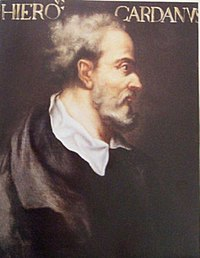
\includegraphics[width=0.50\textwidth]{./images/people/cardano.jpg}
    \end{center}
  \end{column}
\end{columns}


\begin{columns}
  \begin{column}{0.75\textwidth}
   {\small
      The term {\em imaginary} originates from Rene Descartes who considered these
      numbers fictitious and useless!\\
   }
  \end{column}
  \begin{column}{0.25\textwidth}
    \begin{center}
      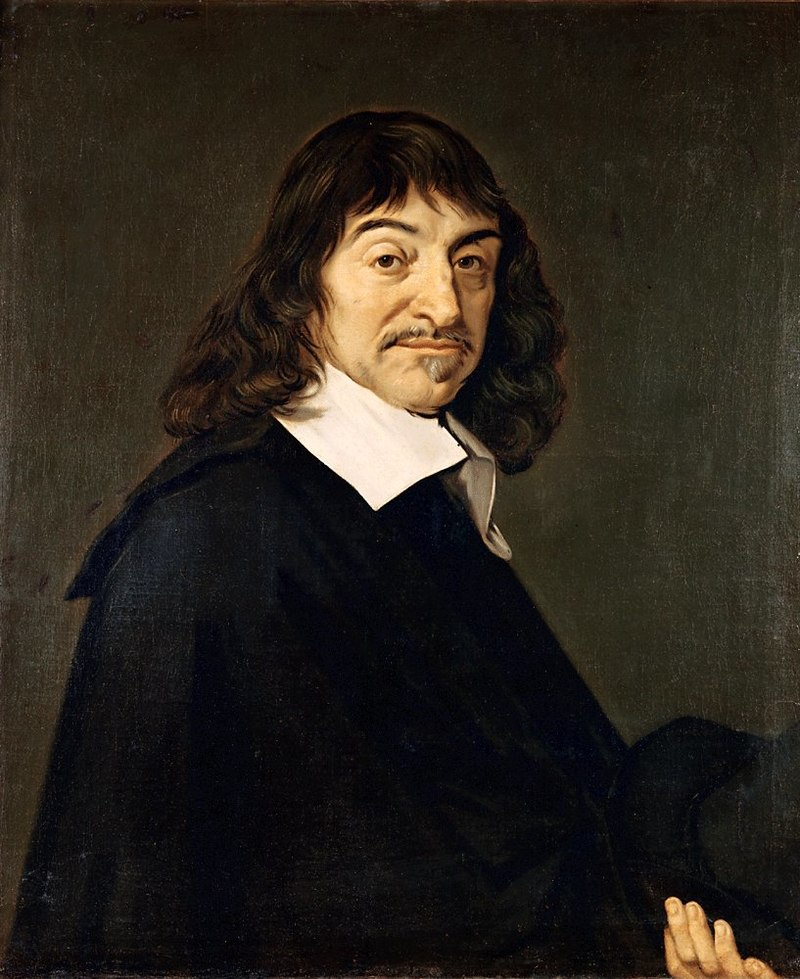
\includegraphics[width=0.50\textwidth]{./images/people/descartes.jpg}
    \end{center}
  \end{column}
\end{columns}


\begin{columns}
  \begin{column}{0.75\textwidth}
   {\small
      {\em Imaginary} numbers became widely accepted through the work of Cauchy, Euler and Gauss.\\
   }
  \end{column}
  \begin{column}{0.25\textwidth}
  \end{column}
\end{columns}

\end{frame}


%
%
%

\begin{frame}{Reminder: Complex numbers}

We define a {\bf complex} number as
\begin{equation*}
  z = x + i y
\end{equation*}
where x, y are real numbers and $i=\sqrt{-1}$.\\

\vspace{0.3cm}
The real part of z, written as $\operatorname{Re}(z)$ (or $\Re(z)$), is x.\\

\vspace{0.3cm}
The imaginary part of z, written as $\operatorname{Re}(z)$ (or $\Im(z)$), is y.\\
\begin{itemize}
  \item Note: The imaginary part is a real number.
\end{itemize}

\vspace{0.3cm}
Therefore, z can be written as
\begin{equation*}
  z = \Re(z) + i \Im(z)
\end{equation*}

\end{frame}

%
%
%

\begin{frame}{Reminder: Complex plane}

\begin{center}
  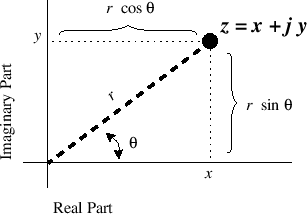
\includegraphics[width=0.50\textwidth]{./images/schematics/complex_plane}
\end{center}

\begin{equation*}
  z = x + i y = r cos\theta + i r sin\theta = r e^{i \theta}
\end{equation*}

\end{frame}


%
%
%

\begin{frame}{Reminder: Complex numbers in polar coordinates}

A complex number z can be represented in polar coordinates as
\begin{equation*}
  z = r e^{i \theta}
\end{equation*}
where r is the magnitude of z and $\theta$ is the angle of z
with respect to the real axis.\\

\vspace{0.3cm}
Using polar coordinates simplifies multiplication
and division:

\begin{equation*}
  z_1 z_2 = r_1 r_2 e^{i (\theta_1 + \theta_2)}
\end{equation*}

\begin{equation*}
  \frac{z_1}{z_2} = \frac{r_1}{r_2} e^{i (\theta_1 - \theta_2)}
\end{equation*}

\end{frame}


} % ending reminder


%
%
%

\begin{frame}{Complex representation of EM waves}

Previously, we studied monochromatic
(single frequency = single "colour") EM waves propagating in the +z
direction, that had no x or y dependence:
\begin{equation*}
    \vec{E}(\vec{r},t) = E_0 cos\Big(kz-\omega t \Big) \hat{x} \;\;\; and \;\;\;
    \vec{B}(\vec{r},t) = B_0 cos\Big(kz-\omega t \Big) \hat{y}
\end{equation*}

\begin{center}
  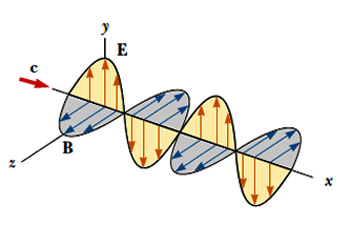
\includegraphics[width=0.20\textwidth]{./images/schematics/emwave_01.jpg}\\
\end{center}

In the above expressions, $E_0$ and $B_0$ are the wave amplitudes,
$\omega$ is the wave's angular frequency, and k is the wave number.\\
\begin{itemize}
  \item k is related to the wavelength $\lambda$ via $k = 2\pi/\lambda$\\
  \item $\omega$ and k are related to the wave velocity c via $c = \omega/k$
\end{itemize}

\vspace{0.3cm}
These are called {\bf plane waves}:
Have no dependence on the position on the plane perpendicular to the direction of travel.

\end{frame}


%
%
%

\begin{frame}{Complex representation of EM waves}

Previously, we studied monochromatic
(single frequency = single "colour") EM waves propagating in the +z
direction, that had no x or y dependence:
\begin{equation*}
    \vec{E}(\vec{r},t) = E_0 cos\Big(kz-\omega t \Big) \hat{x} \;\;\; and \;\;\;
    \vec{B}(\vec{r},t) = B_0 cos\Big(kz-\omega t \Big) \hat{y}
\end{equation*}


The above are the {\bf real parts} of:
\begin{equation*}
    {\color{magenta} \vec{E}(\vec{r},t) = \vec{E}_0  e^{i (kz-\omega t)}  }
    \;\;\; and \;\;\;
    {\color{magenta} \vec{B}(\vec{r},t) = \vec{B}_0  e^{i (kz-\omega t)}  }
\end{equation*}

\noindent\rule{2cm}{0.4pt}\\
{
Recall that
\begin{equation*}
  z = x + i y = r cos\theta + i r sin\theta = r e^{i \theta}
\end{equation*}
}

\end{frame}

%
%
%

\begin{frame}{EM waves are transverse}

In vacuum and away from sources ($\rho$ = 0)
\begin{equation*}
    \vec{\nabla} \cdot \vec{E} = 0
    \xRightarrow{{\color{magenta} \vec{E}(\vec{r},t) = \vec{E}_0  e^{i (kz-\omega t)}  }}
\end{equation*}

therefore
\begin{equation*}
  \Big(
   E_{0x} \frac{\partial }{\partial x} +
   E_{0y} \frac{\partial }{\partial y} +
   E_{0z} \frac{\partial }{\partial z}
  \Big) e^{i (kz-\omega t)} = 0
  \Rightarrow
  i k E_{0z} e^{i (kz-\omega t)} = 0
  \Rightarrow
  {\color{magenta} E_{0z} = 0}
\end{equation*}

\vspace{0.3cm}

Similarly, because $\displaystyle \vec{\nabla} \cdot \vec{B} = 0$,
${\color{magenta} B_{0z} = 0}$.\\

\vspace{0.3cm}

Therefore,
the electromagnetic waves are {\bf transverse}
(i.e. perpendicular to the direction of propagation).\\
\vspace{0.2cm}
For a wave propagating in the +z direction:
\begin{equation*}
    \vec{E}_0 = \Big( E_{0x}, E_{0y}, 0 \Big)   \;\;\; and \;\;\;
    \vec{B}_0 = \Big( B_{0x}, B_{0y}, 0 \Big)
\end{equation*}

\end{frame}

%
%
%

\begin{frame}{EM waves are in phase and mutually perpendicular}

Faraday's law:
\begin{equation*}
   \vec{\nabla} \times \vec{E} = - \partial \vec{B} / \partial t
   \xRightarrow{
     {\color{magenta} \vec{E}(\vec{r},t) = \vec{E}_0  e^{i (kz-\omega t)}  }
     \;\;\; and \;\;\;
     {\color{magenta} \vec{B}(\vec{r},t) = \vec{B}_0  e^{i (kz-\omega t)}  }
   }
\end{equation*}

\begin{equation*}
   \vec{\nabla} \times \Big( \vec{E}_0  e^{i (kz-\omega t)} \Big)
   = - \frac{\partial}{\partial t} \Big( \vec{B}_0  e^{i (kz-\omega t)} \Big)
   \xRightarrow{
     {\color{magenta}
      \vec{\nabla} \times (\lambda \vec{A}) = \lambda \vec{\nabla} \times \vec{A} + (\vec{\nabla}\lambda) \times \vec{A}}}
\end{equation*}

\begin{equation*}
   \Big(\vec{\nabla} e^{i (kz-\omega t)} \Big) \times \vec{E_0} =
    - \vec{B}_0 \frac{\partial}{\partial t} \Big( e^{i (kz-\omega t)} \Big) \Rightarrow
\end{equation*}

\begin{equation*}
   \Big(ik \hat{z} \times \vec{E_0} \Big) e^{i (kz-\omega t)} =
    \Big( i\omega \vec{B}_0 \Big) e^{i (kz-\omega t)} \Rightarrow
\end{equation*}

\begin{equation*}
     k \hat{z} \times \vec{E_0} = \omega \vec{B}_0 \Rightarrow
     {\color{magenta} \vec{B}_0 = \frac{k}{\omega} \hat{z} \times \vec{E_0}}
\end{equation*}

Therefore, $\vec{E}$ and $\vec{B}$ are {\bf mutually perpendicular}.

\end{frame}

%
%
%

%\begin{frame}{EM waves are in phase and mutually perpendicular}
%
%\begin{equation*}
%     {\color{magenta} k \hat{z} \times \vec{E_0} = \omega \vec{B}_0} \Rightarrow
%\end{equation*}
%
%\begin{equation*}
%       \left|
%          \begin{array}{ccc}
%             \hat{x} & \hat{y} & \hat{z} \\
%                   0 &       0 &       k \\
%              E_{0x} &  E_{0y} &       0 \\
%          \end{array}
%       \right| = \omega \Big( B_{0x}, B_{0y}, 0 \Big) \Rightarrow
%\end{equation*}
%
%\begin{equation*}
%  k \Big( -E_{0y}, E_{0x}, 0 \Big) =
%  \omega \Big( B_{0x}, B_{0y}, 0 \Big)
%\end{equation*}
%
%Therefore
%\begin{equation*}
%     -k E_{0y} = \omega B_{0x} \;\;\; and \;\;\;
%      k E_{0x} = \omega B_{0y}
%\end{equation*}
%
%which can be written as:
%\begin{equation*}
%       \vec{B}_{0} = \frac{k}{\omega} \Big( \hat{z} \times \vec{E}_0 \Big)
%\end{equation*}
%
%So $\vec{E}$ and $\vec{B}$ are {\bf mutually perpendicular}.
%
%\end{frame}
%

%
%
%

\begin{frame}{Complex representation of EM waves}

Let's start with fields of the general form:
\begin{equation*}
    \vec{E}(\vec{r},t) = \vec{E}_0  e^{i (kz-\omega t)}
    \;\;\; and \;\;\;
    \vec{B}(\vec{r},t) = \vec{B}_0  e^{i (kz-\omega t)}
\end{equation*}

As we have seen:
\begin{equation*}
       \vec{B}_{0} = \frac{k}{\omega} \Big( \hat{z} \times \vec{E}_0 \Big)
\end{equation*}

Hence amplitudes $B_{0}$ and $E_{0}$ are related by:
\begin{equation*}
     B_{0} = \frac{k}{\omega} E_0 = \frac{1}{c} E_0
\end{equation*}

Embedding the above constraints, the fields can be written as:
\begin{equation*}
    {\color{magenta} \vec{E}(\vec{r},t) = \vec{E}_0  e^{i (kz-\omega t)}  }
    \;\;\; and \;\;\;
    {\color{magenta} \vec{B}(\vec{r},t) = \frac{1}{c} \Big( \hat{z}
      \times \vec{E}_0 \Big)  e^{i (kz-\omega t)} = \frac{1}{c} \Big(
      \hat{z} \times \vec{E} \Big) }
\end{equation*}


\end{frame}


%
%
%

\begin{frame}{Generalization for waves travelling in arbitrary direction}

There is nothing special about the z-axis.\\

\vspace{0.2cm}

We can generalise the previous description:\\

\vspace{0.1cm}

Assume a monochromatic plane EM wave traveling along the
propagation vector $\vec{k}$.
Then $\vec{k} \vec{r}$ is the generalisation of $kz$ and we can write the electric
and magnetic waves as:
\begin{equation*}
     {\color{magenta} \vec{E}(\vec{r},t) = E_0  e^{i (\vec{k} \vec{r} -\omega t)} \hat{n} }
\end{equation*}

and
\begin{equation*}
     {\color{magenta}
           \vec{B}(\vec{r},t) =
                \frac{1}{c}  \Big( \hat{k} \times \vec{E} \Big) =
                \frac{E_0}{c}  e^{i ( \vec{k} \vec{r} -\omega t)} \Big( \hat{k} \times \hat{n} \Big)
     }
\end{equation*}

\vspace{0.3cm}
where $\hat{n}$ is the {\bf polarization vector}, which determines the direction of oscillation of
the electric field.


\end{frame}

%
%
%

\begin{frame}{Polarization}

The expression
\begin{equation*}
     {\color{magenta} \vec{E}(\vec{r},t) = E_0  e^{i (\vec{k} \vec{r} -\omega t)} \hat{n} }
\end{equation*}

describes wave with its electric field vector always along the direction
of $\hat{n}_a = \hat{n}$: This is a {\bf linearly polarised} wave.\\

\vspace{0.3cm}
Evidently, there exists another electric wave, with direction $\hat{n}_b \ne \hat{n}_a$
that is \underline{linearly independent}.\\

\vspace{0.3cm}
Therefore, the most general plane wave can be written as
\begin{equation*}
     {\color{magenta} \vec{E}(\vec{r},t) =
        \Big( E_{0a}(\vec{r},t) \hat{n}_a + E_{0b}(\vec{r},t) \hat{n}_b \Big)  e^{i (\vec{k} \vec{r} -\omega t)}  }
\end{equation*}

\vspace{0.3cm}
In principle, the amplitudes $E_{0a}$ and $E_{0b}$ are complex numbers,
allowing the possibility of a phase difference between the 2 linearly independent waves.

\end{frame}

%
%
%

\begin{frame}{Polarization}

The most general plane wave can be written as
\begin{equation*}
     {\color{magenta} \vec{E}(\vec{r},t) =
        \Big( E_{0a}(\vec{r},t) \hat{n}_a + E_{0b}(\vec{r},t) \hat{n}_b \Big)  e^{i (\vec{k} \vec{r} -\omega t)}  }
\end{equation*}

If $E_{0a}$ and $E_{0b}$ have the {\bf same phase},
they yield a {\bf linearly polarised} wave.

The wave has a polarization vector forming an
angle $\theta$ with respect to $\hat{n}_a$
\begin{equation*}
  tan\theta = E_{0b} / E_{0a}
\end{equation*}

The magnitude of that wave is given by
\begin{equation*}
  E_0 = \sqrt{E_{0b}^2 + E_{0a}^2}
\end{equation*}

\end{frame}

%
%
%

\begin{frame}{Polarization}

The most general plane wave can be written as
\begin{equation*}
     {\color{magenta} \vec{E}(\vec{r},t) =
        \Big( E_{0a}(\vec{r},t) \hat{n}_a + E_{0b}(\vec{r},t) \hat{n}_b \Big)  e^{i (\vec{k} \vec{r} -\omega t)}  }
\end{equation*}

If the coplex amplitudes $E_{0a}$ and $E_{0b}$ have a {\bf phase difference},
they yield an {\bf elliptically polarised} wave.\\

\vspace{0.2cm}

In the special case where the phase difference is 90$^o$,
and $E_{0a}$ = $E_{0b}$, we have a {\bf circularly polarised} wave.

\begin{equation*}
     {\color{magenta} \vec{E}(\vec{r},t) =
        E_{0a}(\vec{r},t) \Big(  \hat{n}_a + i \hat{n}_b \Big)  e^{i (\vec{k} \vec{r} -\omega t)}  }
\end{equation*}

\begin{center}
    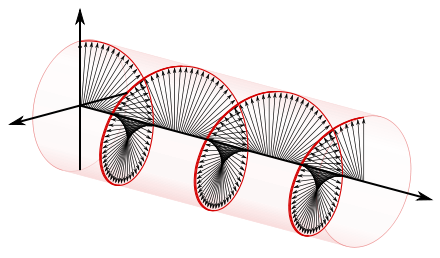
\includegraphics[width=0.40\textwidth]{./images/schematics/wave_circular_polarization.png}
\end{center}

\end{frame}

%
%
%

\begin{frame}{Polarization}

If it also possible that the direction of the polarization vector is
{\bf random in time}: In this case we have an {\bf unpolarized} EM wave.

\begin{center}
    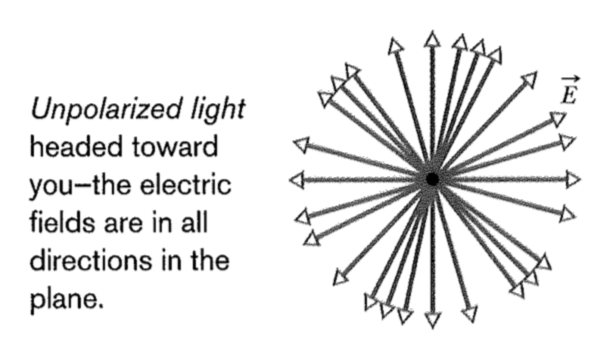
\includegraphics[width=0.60\textwidth]{./images/schematics/unpolarised_light_heading_towards_you.png}
\end{center}

\end{frame}

%
%
%

\begin{frame}{Intensity of transmitted polarized light}

\begin{columns}
  \begin{column}{0.40\textwidth}
    \begin{center}
       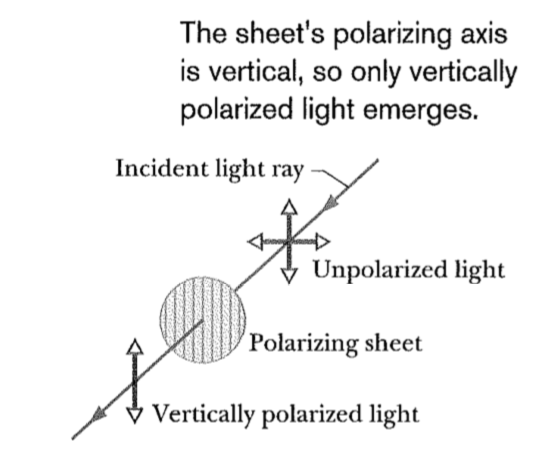
\includegraphics[width=0.90\textwidth]{./images/schematics/unpolarized_light_sent_through_filter.png}\\
    \end{center}
  \end{column}
  \begin{column}{0.60\textwidth}
      We can transform unpolarized visible light into polarized light by passing
      it through a {\bf polarizing sheet}.\\
      \vspace{0.2cm}
      If $I_0$ is the intensity of the unpolarized light,
      the intensity $I$ of the transmitted light is:
      \begin{equation*}
        I = \frac{1}{2}I_0
      \end{equation*}
  \end{column}
\end{columns}

\begin{columns}
  \begin{column}{0.40\textwidth}
    \begin{center}
       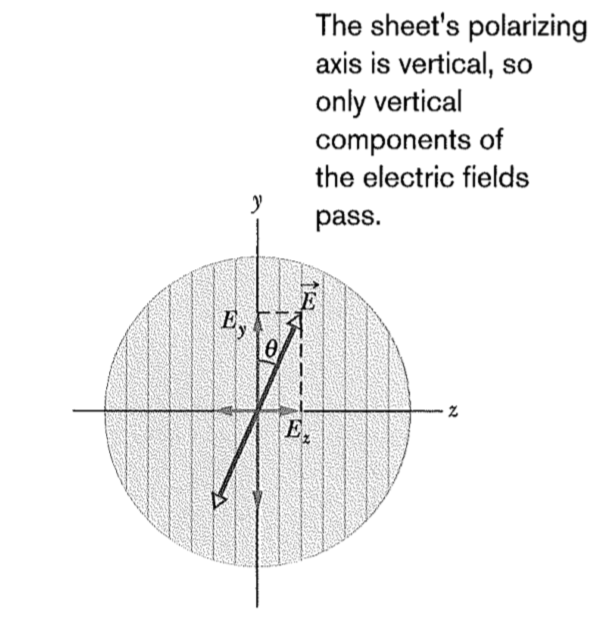
\includegraphics[width=0.75\textwidth]{./images/schematics/polarized_light_sent_through_filter.png}\\
    \end{center}
  \end{column}
  \begin{column}{0.60\textwidth}
      If the light reaching the filter is already polarized,
      the intensity $I$ of the transmitted light is:
      \begin{equation*}
        I = I_0 cos^2\theta
      \end{equation*}
      where $\theta$ is the angle between the electric field $\vec{E}$
      and the polarizing direction of the sheet.
  \end{column}
\end{columns}


\end{frame}


%...............................................................................

%
% Worked example
%

{
\problemslide

\begin{frame}{Worked example}

\begin{blockexmplque}{Question}
  Initially unpolarized light is sent into a system
  of three polarizing sheets, as shown in the figure below,
  whose polarizing directions make angles
  of $\theta_1$ = $\theta_2$ = $\theta_3$ = $50^o$ with
  the direction of the $y$ axis. What percentage
  of the initial intensity is transmitted by the system?\\

  \begin{center}
   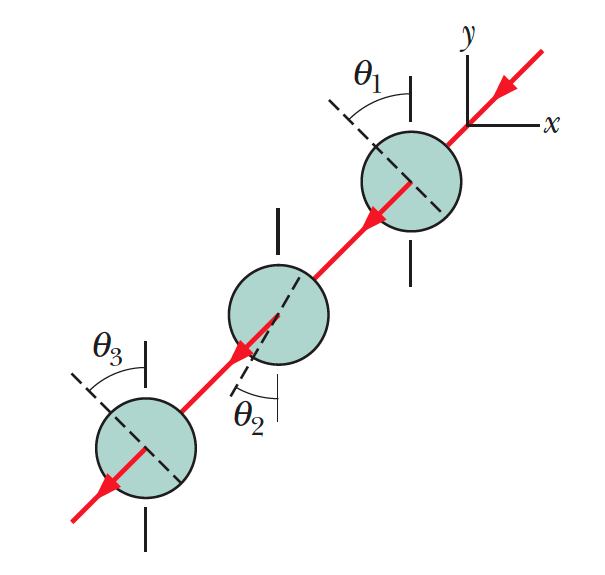
\includegraphics[width=0.35\textwidth]{./images/problems/lect10_3filters}\\
  \end{center}
\end{blockexmplque}

\end{frame}

%
%
%
%

\begin{frame}{Worked example}

  After passing through the first polarizer the initial intensity $I_0$
  reduces by a factor of 1/2.

  After passing through the second one it is further reduced by a factor of
  \begin{equation*}
   cos^2(\pi - \theta_1 - \theta_2) = cos^2(\theta_1 + \theta_2).
  \end{equation*}

  Finally, after passing through the third one it is again reduced by
  a factor of
  \begin{equation*}
   cos^2(\pi - \theta_2 - \theta_3) = cos^2(\theta_2 + \theta_3).
  \end{equation*}

  Therefore, the ratio of the final intensity $I_f$ to the the initial intensity $I_0$
  is given by:

  \begin{equation*}
     \frac{I_f}{I_0} = \frac{1}{2} cos^2(\theta_1 + \theta_2) cos^2(\theta_2 + \theta_3) = 4.5 \times 10^{-4}
  \end{equation*}

\end{frame}

} % \problemslide

%...............................................................................

%
%
%

\begin{frame}{Applications of polarized light}

Many practical applications in science, industry and every-day life.

\begin{itemize}
  \item in geology:
     \begin{itemize}
           \item mineral identification
     \end{itemize}
  \item in chemistry:
     \begin{itemize}
           \item determining chirality of organic compounds,
     \end{itemize}
  \item in astronomy:
     \begin{itemize}
            \item information on the source of radiation, interstellar dust clouds and magnetic fields.
            \item physics of early universe
     \end{itemize}
  \item in 3D films, LCD TVs, sunglasses

\end{itemize}

\end{frame}


%
%
%

\begin{frame}{Skylight polarization - Polarization by scattering}

\begin{center}
   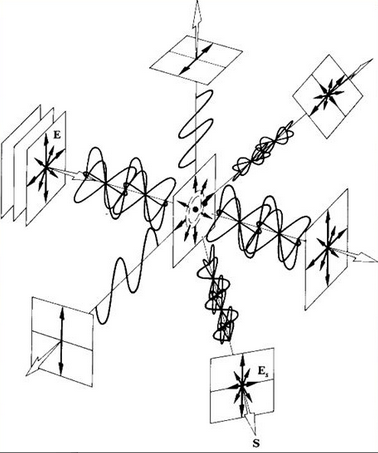
\includegraphics[width=0.50\textwidth]{./images/schematics/skylight_polarization_scattering.png}\\
\end{center}

\end{frame}

%
%
%

\begin{frame}{Skylight polarization}

You can easily observe the polarization of the skylight using a simple linear polarizer.

\begin{columns}
  \begin{column}{0.47\textwidth}
    \begin{center}
       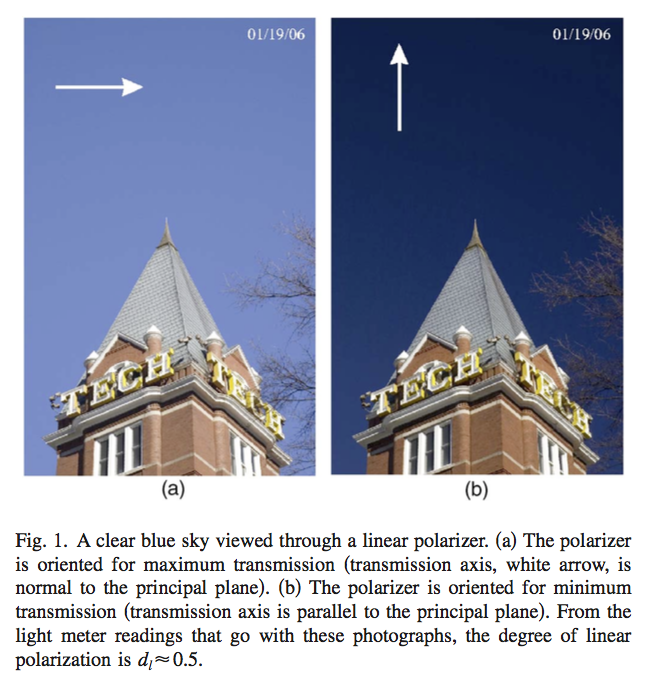
\includegraphics[width=0.90\textwidth]{./images/photos/skylight_polarization.png}\\
       {\tiny
           from G.S. Smith, Am. J. Phys 75 (1), January 2007
       }
    \end{center}
  \end{column}
  \begin{column}{0.53\textwidth}
      \begin{itemize}
       {\small
         \item Sunlight is scattered by aerosols as it propagates through the atmosphere.
         \item Scattered light is partially polarised.
         \item Effect stronger at points in the sky at a $\pi/2$ angle wrt the Sun.
         \item Insects can detect polarized light and use it for orientation.
         \item The human eye has marginal sensitivity to polarization.
         \item It is alleged that Vikings used naturally occurring (mineral) polarizing filters
                   to navigate using the Sun even with an overcast sky.
       }
      \end{itemize}
  \end{column}
\end{columns}

\end{frame}

%
%
%

\begin{frame}{Light polarization \& sunglasses}

\begin{columns}
  \begin{column}{0.45\textwidth}
    \begin{center}
       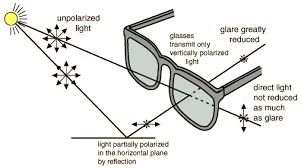
\includegraphics[width=0.90\textwidth]{./images/schematics/sunglass_polarization_principle.png}\\
       {\tiny
           hyperphysics.phy-astr.gsu.edu
       }
    \end{center}
  \end{column}
  \begin{column}{0.55\textwidth}
     Polarized sunglass lenses reduce reflected glare.\\
  \end{column}
\end{columns}

\begin{columns}
  \begin{column}{0.50\textwidth}
    \begin{center}
       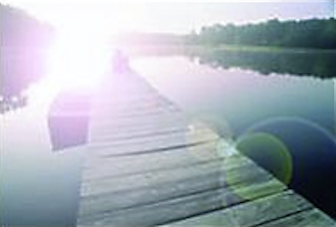
\includegraphics[width=0.75\textwidth]{./images/photos/lake_without_polarized_lenses.png}\\
       {\tiny
           Without polarized lenses.
       }
    \end{center}
  \end{column}
  \begin{column}{0.50\textwidth}
    \begin{center}
       
\includegraphics[width=0.75\textwidth]{./images/photos/lake_with_polarized_lenses.png}\\
       {\tiny
           With polarized lenses.
       }
    \end{center}
  \end{column}
\end{columns}

\end{frame}

%
%
%

\begin{frame}{Light polarization \& LCD TVs}

\begin{columns}
  \begin{column}{0.60\textwidth}
    {\scriptsize
     Pixels between polarization filters, normally appear dark.
     Liquid crystal that can be turned on electronically rotates the light by $\pi/2$
     allowing light to flow through the two filters and making the pixel appear bright.
    }
    \begin{center}
       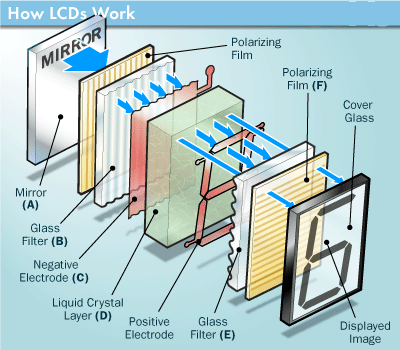
\includegraphics[width=0.80\textwidth]{./images/schematics/how_lcds_work.png}\\
    \end{center}
  \end{column}
  \begin{column}{0.40\textwidth}
       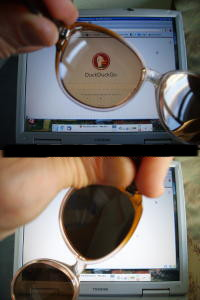
\includegraphics[width=0.90\textwidth]{./images/photos/polarized_light_lcd_display.jpg}\\
  \end{column}
\end{columns}

\end{frame}


%
%
%

\begin{frame}{Working towards the most general set of equations}

\begin{center}
    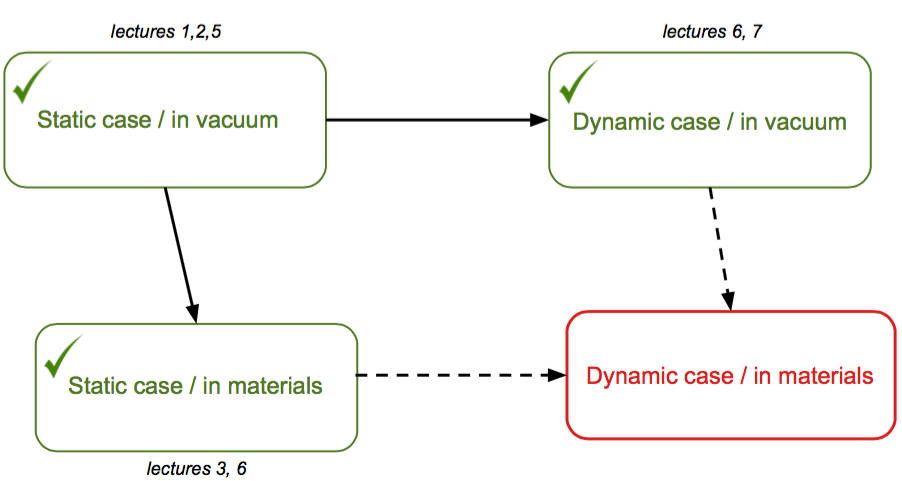
\includegraphics[width=0.95\textwidth]{./images/schematics/maxwell_eq_variations_2.png}\\
\end{center}

\end{frame}

%
%
%

\begin{frame}{Maxwell's equations}

{\small

 \begin{center}
 {

  %
  %
  \begin{columns}
    \begin{column}{0.20\textwidth}

       For a linear medium:
       \begin{equation*}
          \vec{D} = \epsilon \vec{E}
       \end{equation*}
       \begin{equation*}
          \vec{H} = \frac{\vec{B}}{\mu}
       \end{equation*}

    \end{column}
    \begin{column}{0.80\textwidth}

  \begin{table}[H]
    \begin{tabular}{|l|c|c|}
      \hline
        \multicolumn{3}{|l|} {
          {\color{magenta}
           {\bf Static case in matter}
          }
        }\\
      \hline
      {\bf Gauss's law} &
        $\displaystyle \oint \vec{D} \cdot d\vec{S} =  \int \rho_{f} d\tau$ &
        $\displaystyle \vec{\nabla} \cdot \vec{D} = \rho_{f}$ \\

      {\bf Circuital law} &
        $\displaystyle \oint \vec{E} \cdot d\vec{\ell} = 0$ &
        $\displaystyle \vec{\nabla} \times \vec{E} = 0$ \\

      {\bf Gauss's law} (magn.) &
        $\displaystyle \oint \vec{B} \cdot d\vec{S} = 0$ &
        $\displaystyle \vec{\nabla} \cdot \vec{B} = 0$ \\

      {\bf Ampere's law} &
        $\displaystyle \oint \vec{H} \cdot d\vec{\ell} =  \int \vec{j}_{f} \cdot d\vec{S}$ &
        $\displaystyle \vec{\nabla} \times \vec{H} = \vec{j}_{f}$ \\
      \hline
    \end{tabular}
  \end{table}

    \end{column}
  \end{columns}

  %
  %
  \begin{table}[H]
    \begin{tabular}{|l|c|c|}
      \hline
        \multicolumn{3}{|l|} {
          {\color{magenta}
           {\bf Dynamic case in vacuum}
          }
        }\\
      \hline
      {\bf Gauss's law} &
        $\displaystyle \oint \vec{E} \cdot d\vec{S} = \frac{1}{\epsilon_0} \int \rho d\tau$ &
        $\displaystyle \vec{\nabla} \cdot \vec{E} = \frac{\rho}{\epsilon_0}$ \\

      {\bf Faraday's law} &
        $\displaystyle \oint \vec{E} \cdot d\vec{\ell} =  -\frac{\partial}{\partial t} \int \vec{B} d\vec{S}$ &
        $\displaystyle \vec{\nabla} \times \vec{E} = -  \frac{\partial \vec{B}}{\partial t}$ \\

      {\bf Gauss's law} (magn.) &
        $\displaystyle  \oint \vec{B} \cdot d\vec{S} = 0$ &
        $\displaystyle  \vec{\nabla} \cdot \vec{B} = 0$ \\

      {\bf Ampere's law} &
        $\displaystyle \oint \vec{B} \cdot d\vec{\ell} = \mu_{0} \int \Big( \vec{j} + \epsilon_0 \frac{\partial \vec{E}}{\partial t}\Big) \cdot d\vec{S}$ &
        $\displaystyle \vec{\nabla} \times \vec{B} = \mu_{0} \Big( \vec{j} + \epsilon_0 \frac{\partial \vec{E}}{\partial t}\Big)$ \\
      \hline
    \end{tabular}
  \end{table}

 }
 \end{center}

}

\end{frame}

%
%
%

\begin{frame}{Maxwell's equations}

{\small

\setlength{\extrarowheight}{12pt}
\setlength{\arraycolsep}{5pt}

 \begin{center}
 {

  \begin{table}[H]
    \begin{tabular}{|l|c|c|}
      \hline
        \multicolumn{3}{|l|} {
          {\color{magenta}
           {\bf Dynamic case in matter}
          }
        }\\
      \hline
      {\bf Gauss's law} &
        $\displaystyle \oint \vec{D} \cdot d\vec{S} = \int \rho_f d\tau = Q_f$   &
        $\displaystyle \vec{\nabla} \cdot \vec{D} = \rho_f$ \\

      {\bf Faraday's law} &
        $\displaystyle \oint \vec{E} \cdot d\vec{\ell} = -\frac{\partial}{\partial t} \int \vec{B} \cdot d\vec{S} \Rightarrow$ &
        $\displaystyle \vec{\nabla} \times \vec{E} = -  \frac{\partial \vec{B}}{\partial t}$ \\
      &
        $\displaystyle \oint \vec{E} \cdot d\vec{\ell} = -\frac{d\Phi_B}{dt}$ & \\

      {\bf Gauss's law} (magn.) &
        $\displaystyle  \oint \vec{B} \cdot d\vec{S} = 0$ &
        $\displaystyle  \vec{\nabla} \cdot \vec{B} = 0$ \\

      {\bf Ampere's law} &
        $\displaystyle \oint \vec{H} \cdot d\vec{\ell} =
           \int_{S} \Big( \vec{j} + \frac{\partial \vec{D}}{\partial t}\Big) \cdot d\vec{S} \Rightarrow$ &
        $\displaystyle \vec{\nabla} \times \vec{H} = \vec{j}_f + \frac{\partial \vec{D}}{\partial t}$ \\
      &
        $\displaystyle \oint \vec{H} \cdot d\vec{\ell} = I_f + \frac{d\Phi_D}{dt}$ & \\
      \hline
    \end{tabular}
  \end{table}

 }
 \end{center}
}

\end{frame}


%
%
%

\begin{frame}{EM waves in matter}

In an earlier lecture, I solved the time-dependent Maxwell's equations in vacuum and in absence
of sources. We saw that the solutions were (EM) waves!\\

\vspace{0.2cm}

Now I plan to do something similar, but starting from the time-dependent Maxwell's
equations in matter. In absence of sources we have:\\
\begin{equation*}
    \vec{\nabla} \cdot \vec{D} = \cancel{\rho_f} \Rightarrow
    \vec{\nabla} \cdot \vec{D} = 0
\end{equation*}

\begin{equation*}
    \vec{\nabla} \times \vec{E} = -  \frac{\partial \vec{B}}{\partial t}
\end{equation*}

\begin{equation*}
    \vec{\nabla} \cdot \vec{B} = 0
\end{equation*}

\begin{equation*}
    \vec{\nabla} \times \vec{H} = \cancel{\vec{j}_f} + \frac{\partial \vec{D}}{\partial t} \Rightarrow
    \vec{\nabla} \times \vec{H} = \frac{\partial \vec{D}}{\partial t}
\end{equation*}

\end{frame}

%
%
%

\begin{frame}{EM waves in matter}

For a linear medium:
\begin{equation*}
         \vec{D} = \epsilon \vec{E} \;\;\;\; and \;\;\;\; \vec{H} = \frac{\vec{B}}{\mu}
\end{equation*}

Maxwell's equations become:
\begin{equation*}
    \vec{\nabla} \cdot \vec{E} = 0
\end{equation*}

\begin{equation*}
    \vec{\nabla} \times \vec{E} = -  \frac{\partial \vec{B}}{\partial t}
\end{equation*}

\begin{equation*}
    \vec{\nabla} \cdot \vec{B} = 0
\end{equation*}

\begin{equation*}
    \vec{\nabla} \times \vec{B} = \mu \epsilon \frac{\partial \vec{E}}{\partial t}
\end{equation*}

This system of equations is similar with the one we studied in an
earlier lecture, with  $\mu_0 \epsilon_0$ replaced by  $\mu \epsilon$.

\end{frame}

%
%
%

\begin{frame}{EM waves in matter}

So, through a linear medium electromagnetic waves propagate
with velocity:
\begin{equation*}
   u = \frac{1}{\sqrt{\epsilon \mu}}
\end{equation*}

This velocity can be written as:
\begin{equation*}
   u = \frac{1}{\sqrt{\epsilon_0 \mu_0}} \cdot
          \frac{\sqrt{\epsilon_0 \mu_0}}{\sqrt{\epsilon \mu}}
      = \frac{c}{n}
\end{equation*}

where
\begin{equation*}
   n = \frac{\sqrt{\epsilon \mu}}{\sqrt{\epsilon_0 \mu_0}}
\end{equation*}
is the {\bf index of refraction} of the material.

\end{frame}

%
%
%

\begin{frame}{EM waves in matter}

The index of refraction:
\begin{equation*}
   n = \frac{\sqrt{\epsilon \mu}}{\sqrt{\epsilon_0 \mu_0}}
\end{equation*}
can also be written as:
\begin{equation*}
   n = \frac{\sqrt{\epsilon_r \epsilon_0 \mu_r
       \mu_0}}{\sqrt{\epsilon_0 \mu_0}} = \sqrt{\epsilon_r \mu_r}
\end{equation*}

For most materials $\mu_r$ is close to 1 and $\epsilon_r$ is
larger than one and, therefore, almost always $n > 1$.\\

\vspace{0.2cm}

So {\bf light travels in
matter more slowly} than it does in the vacuum!

\vspace{0.2cm}

For example, for water n $\approx$ 1.33 so light slows down by 25\%.

\end{frame}

%
%
%

\begin{frame}{Cherenkov radiation}

\begin{columns}
  \begin{column}{0.70\textwidth}
  {\small
     So, within a medium (but not in vacuum), particles can travel faster than light!\\
     When a charged particle travels faster than the speed of light in a medium,
     it generates an {\bf EM shockwave} called {\bf Cherenkov radiation}.
  }
  \end{column}
  \begin{column}{0.30\textwidth}
    \begin{center}
      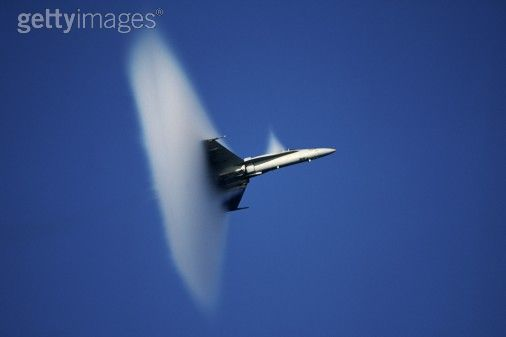
\includegraphics[width=0.90\textwidth]{./images/photos/plane_breaking_sound_wave.jpg}\\
    \end{center}
  \end{column}
\end{columns}

\begin{columns}
  \begin{column}{0.60\textwidth}
    \begin{center}
      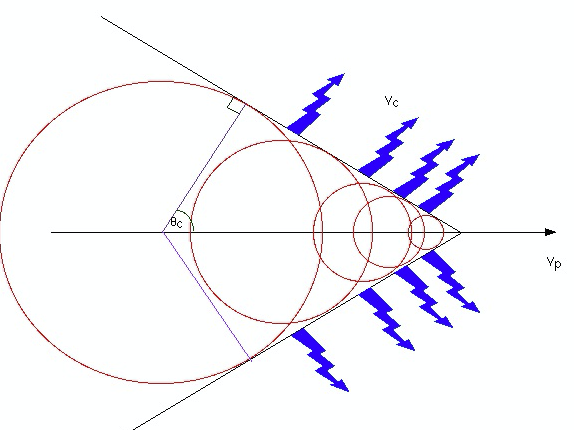
\includegraphics[width=0.90\textwidth]{./images/schematics/cherenkov_cone.png}\\
    \end{center}
  \end{column}
  \begin{column}{0.40\textwidth}
  {\small
      Cherenkov radiation is emitted in a cone with opening angle
      \begin{equation*}
           \theta_C = cos^{-1} \Big( \frac{1}{\beta n} \Big)
      \end{equation*}
      where n is the index of refraction of the medium and $\beta$ is the particle velocity ($\beta=u/c$).
  }
  \end{column}
\end{columns}

\end{frame}

%
%
%

\begin{frame}{Cherenkov radiation}

\begin{columns}
  \begin{column}{0.60\textwidth}
    \begin{center}
      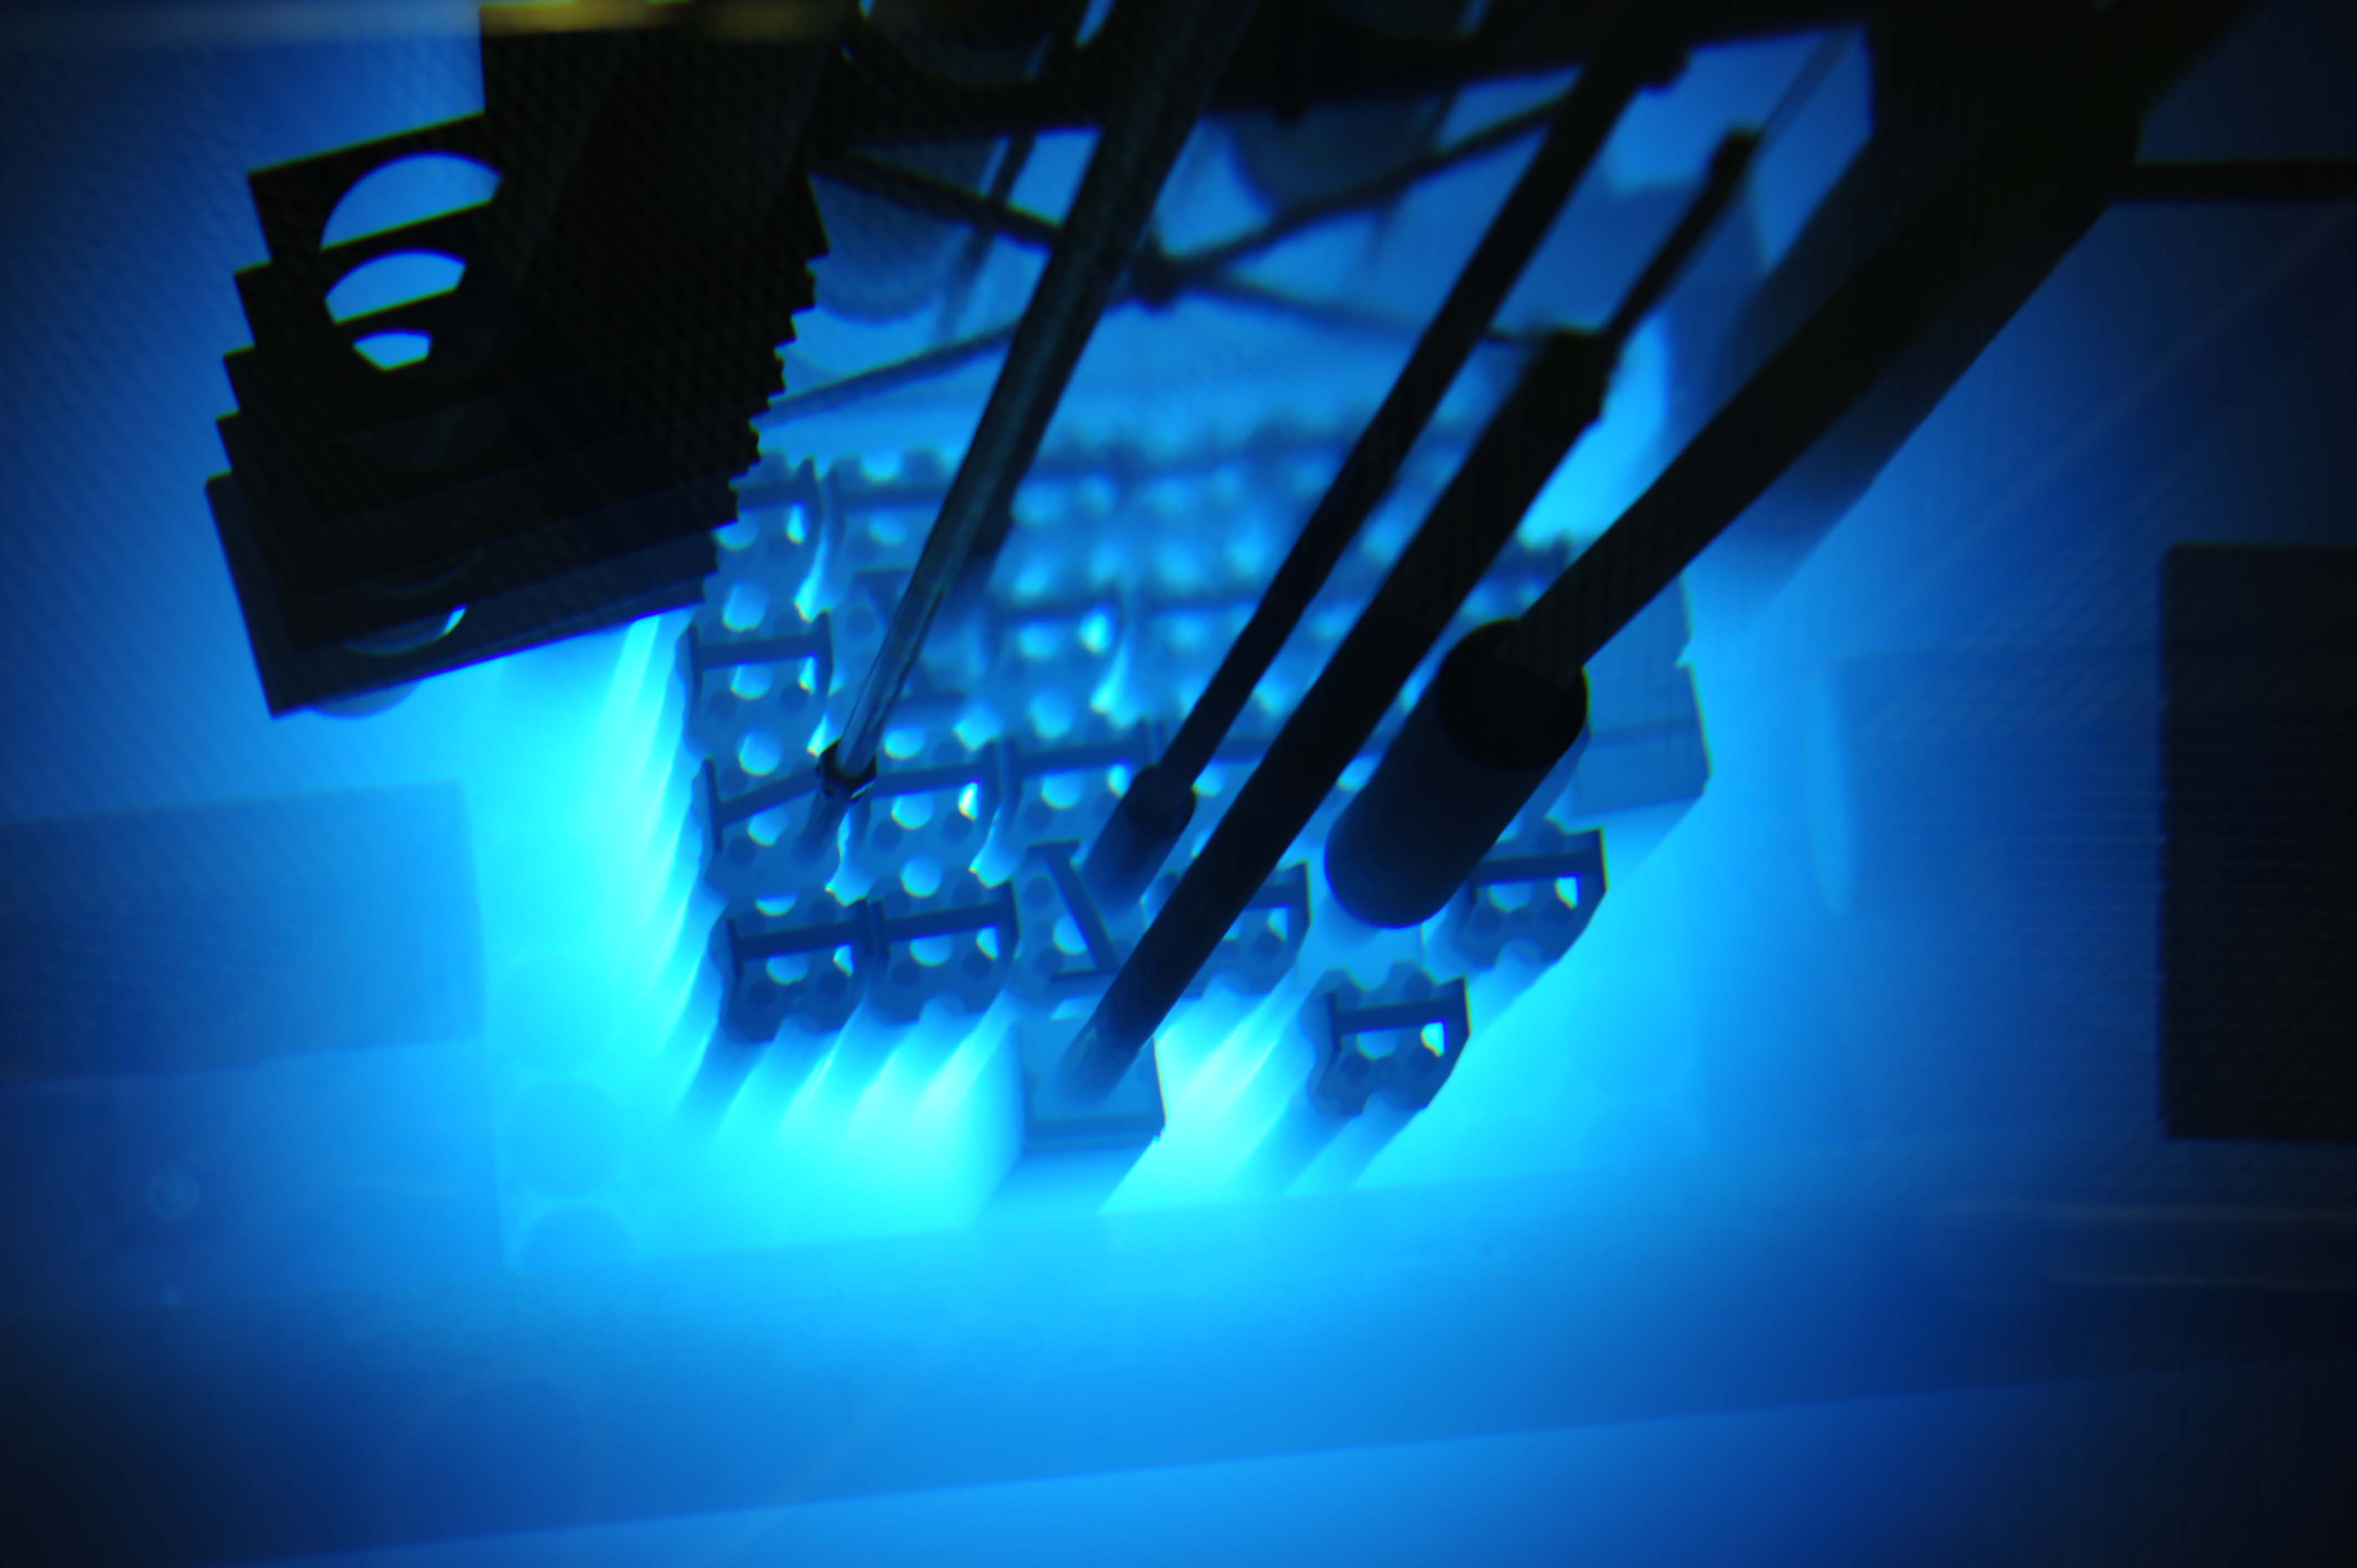
\includegraphics[width=0.90\textwidth]{./images/photos/cherenkov_light.jpg}\\
    \end{center}
  \end{column}
  \begin{column}{0.40\textwidth}
      Cherenkov glow around a pool-type nuclear reactor.
  \end{column}
\end{columns}

\end{frame}


%
%
%

%
%
%

\begin{frame}{Cherenkov radiation}

Cherenkov radiation is being used to detect high-energy gamma ray sources in the universe.

\begin{columns}
  \begin{column}{0.60\textwidth}
    \begin{center}
      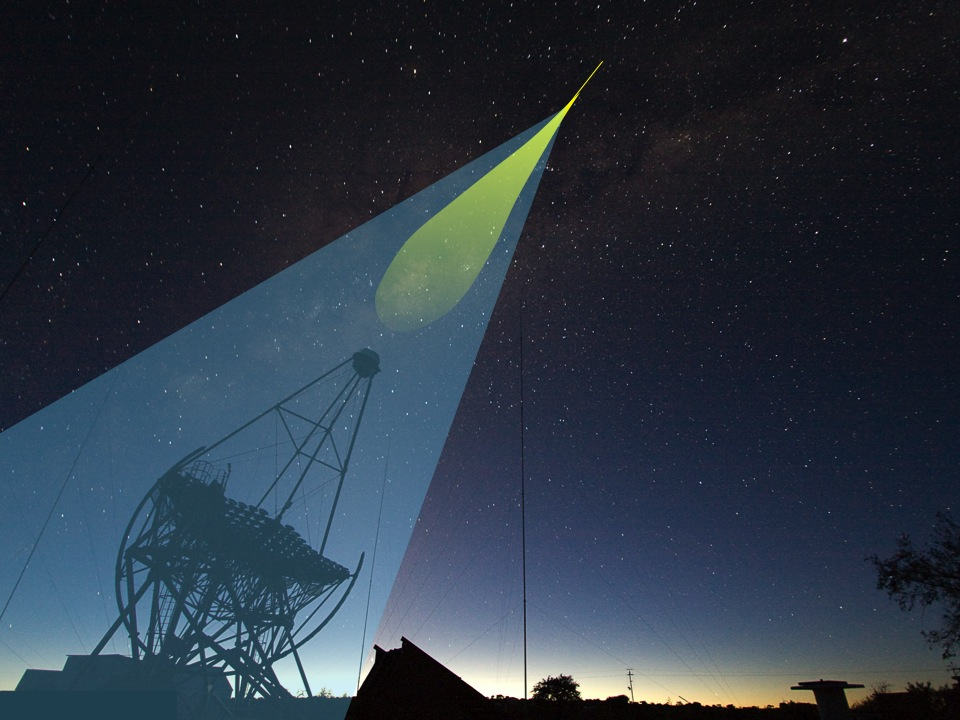
\includegraphics[width=0.90\textwidth]{./images/photos/hess.jpg}\\
    \end{center}
  \end{column}
  \begin{column}{0.40\textwidth}
    \begin{center}
      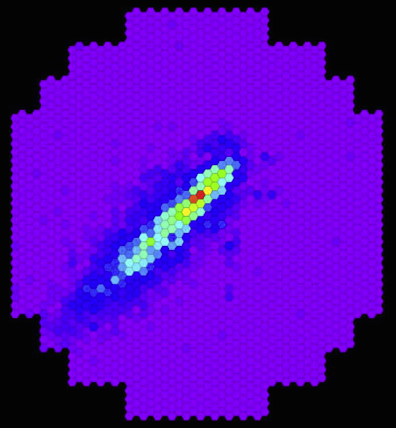
\includegraphics[width=0.90\textwidth]{./images/photos/hess_event_display.png}\\
    \end{center}
  \end{column}
\end{columns}

(HESS - High Energy Stereoscopic System)

\end{frame}

%
%
%

\begin{frame}{Cherenkov radiation}

Cherenkov radiation is also being used to detect man-made (accelerator),
atmospheric and solar neutrinos [Nobel prize in Physics 2002 and 2015]

\begin{columns}
  \begin{column}{0.40\textwidth}
    \begin{center}
      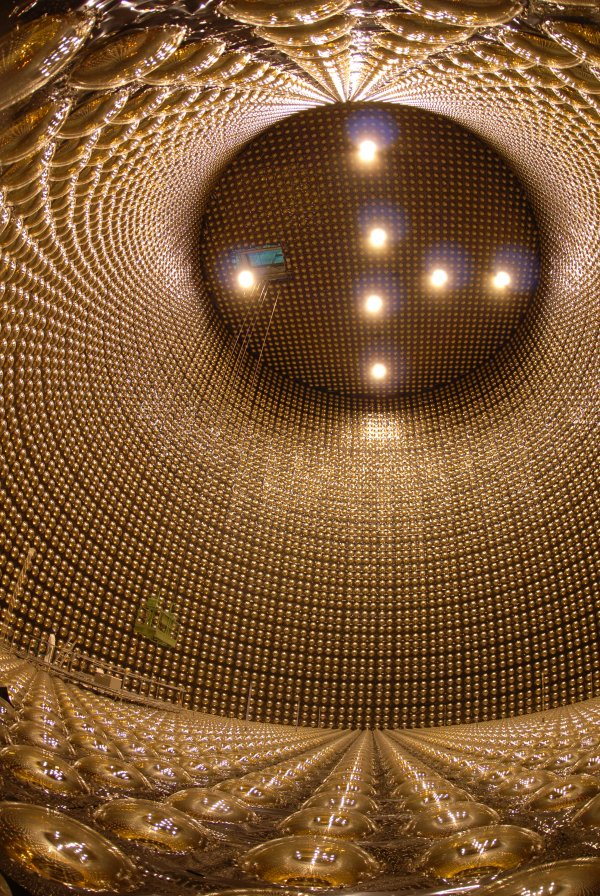
\includegraphics[width=0.80\textwidth]{./images/photos/superk.jpg}\\
    \end{center}
  \end{column}
  \begin{column}{0.60\textwidth}
    \begin{center}
      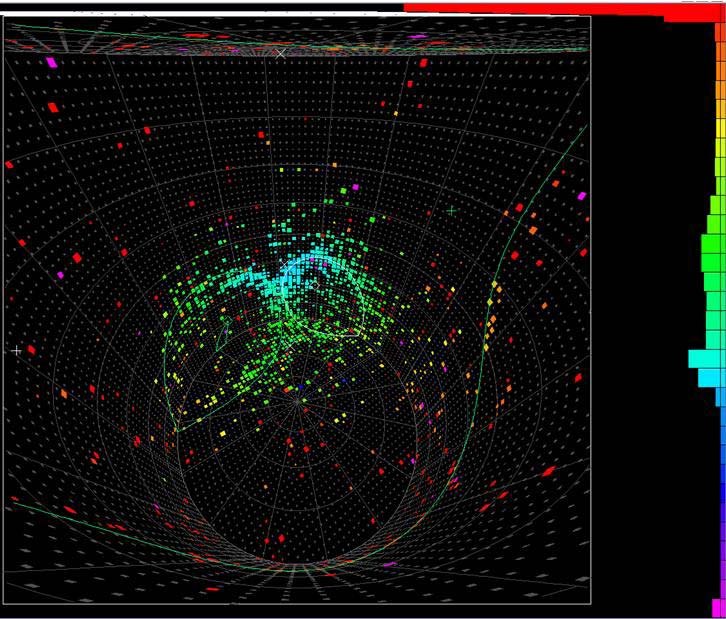
\includegraphics[width=0.90\textwidth]{./images/photos/superk_event_display.jpg}\\
    \end{center}
  \end{column}
\end{columns}

(Super-Kamiokande detector)

\end{frame}


%
%
%

\begin{frame}{EM waves at the boundary of transparent media}

\begin{columns}
  \begin{column}{0.50\textwidth}
    \begin{center}
      
\includegraphics[width=0.90\textwidth]{./images/photos/pencil_in_glass_of_water.jpg}\\
    \end{center}
  \end{column}
  \begin{column}{0.50\textwidth}
      What happens when a wave crosses the {\bf boundary between two transparent media}?\\
      \vspace{0.5cm}
      To examine what exactly happens we need to understand the
      electrodynamic boundary conditions.
  \end{column}
\end{columns}

\end{frame}

%
%
%

\begin{frame}{Boundary conditions for the electric field}

\begin{columns}
  \begin{column}{0.50\textwidth}
   {\small
     Assume that the boundary between two dielectrics (with
     permittivities $\epsilon_1$ and  $\epsilon_2$)
     is carrying surface charge density $\sigma_f$.\\
     Consider the volume shown around the surface and
     assume that the height is infinitesimally small so the side
     surfaces can be ignored.
  }
  \end{column}
  \begin{column}{0.50\textwidth}
    \begin{center}
      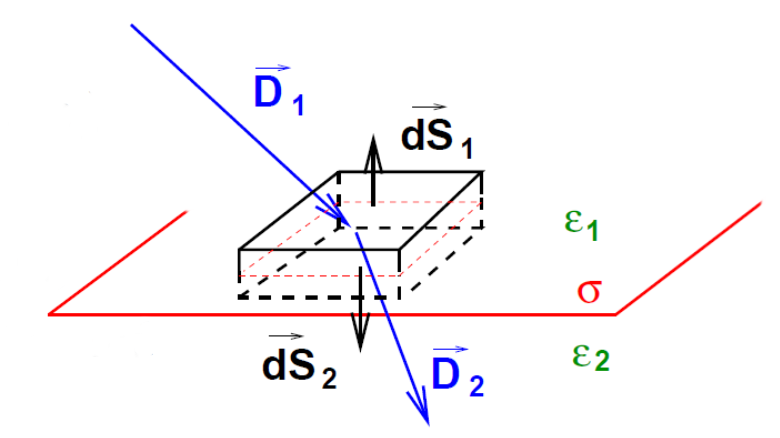
\includegraphics[width=0.95\textwidth]{./images/schematics/boundary_conditions_electric_field_1.png}\\
    \end{center}
  \end{column}
\end{columns}

\begin{equation*}
  \oint \vec{D} \cdot d\vec{S} = Q_f \Rightarrow
       %\vec{D}_1 \vec{S}_1 + \vec{D}_2 \vec{S}_2 = Q_f \Rightarrow
       D_2^{\perp} S - D_1^{\perp} S = Q_f \xRightarrow{Q_f = \sigma_f S}
%         {\color{magenta}D_2^{\perp} - D_1^{\perp} = \sigma_f}
\end{equation*}
\begin{equation*}
         {\color{magenta}D_2^{\perp} - D_1^{\perp} = \sigma_f}
\end{equation*}

The electric displacement $\vec{D}$ is given by
$\displaystyle \vec{D} = \epsilon \vec{E}$,
therefore:
\begin{equation*}
   \epsilon_2 \vec{E}_2^{\perp} - \epsilon_1 \vec{E}_1^{\perp} = \sigma
\end{equation*}

In the absence of free charges ($\sigma_f=0$):
\begin{equation*}
   {\color{magenta} \epsilon_1 \vec{E}_1^{\perp} = \epsilon_2 \vec{E}_2^{\perp} }
\end{equation*}

\end{frame}


%
%
%

\begin{frame}{Boundary conditions for the electric field}

\begin{columns}
  \begin{column}{0.50\textwidth}
   {\small
     Again, assume that the boundary between two dielectrics (with
     permittivities $\epsilon_1$ and  $\epsilon_2$)
     is carrying surface charge density $\sigma$.\\
     Consider the path shown around the surface and
     assume that the height is infinitesimally small so the perpendicular
     sides can be ignored.
  }
  \end{column}
  \begin{column}{0.50\textwidth}
    \begin{center}
      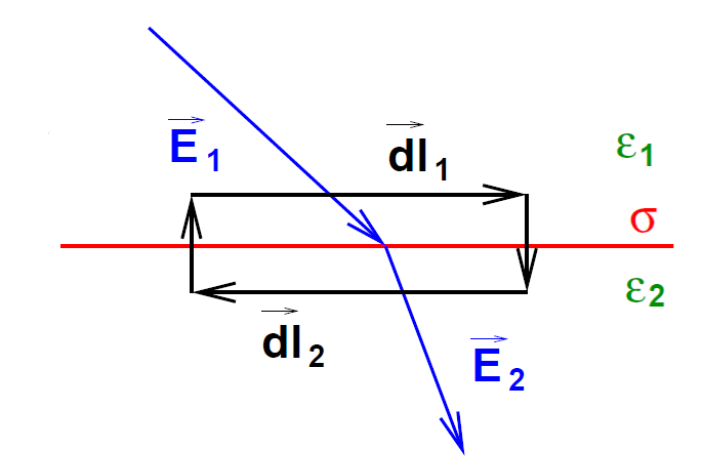
\includegraphics[width=0.95\textwidth]{./images/schematics/boundary_conditions_electric_field_2.png}\\
    \end{center}
  \end{column}
\end{columns}

\begin{equation*}
  \oint \vec{E} \cdot d\vec{\ell} = 0 \Rightarrow
       %\vec{E}_1 \vec{\ell}_1 + \vec{E}_2 \vec{\ell}_2 = 0 \Rightarrow
       E_1^{\parallel} \ell - E_2^{\parallel} \ell = 0 \Rightarrow
         {\color{magenta} E_1^{\parallel} = E_2^{\parallel}}
\end{equation*}

\end{frame}

%
%
%

\begin{frame}{Boundary conditions for the magnetic field}

\begin{columns}
  \begin{column}{0.50\textwidth}
  {\small
     Assume that the boundary between two materials (with
     permeabilities $\mu_1$ and  $\mu_2$)
     is carrying surface current density $\vec{j}_f$.\\
     Consider the volume shown around the surface and
     assume that the height is infinitesimally small so the side
     surfaces can be ignored.
  }
  \end{column}
  \begin{column}{0.50\textwidth}
    \begin{center}
      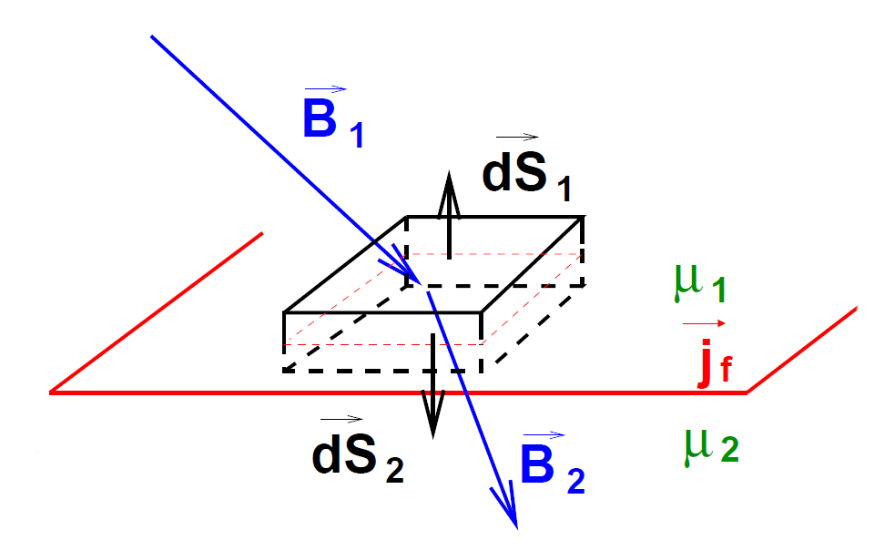
\includegraphics[width=0.95\textwidth]{./images/schematics/boundary_conditions_magnetic_field_1.png}\\
    \end{center}
  \end{column}
\end{columns}

\begin{equation*}
  \oint \vec{B} \cdot d\vec{S} = 0 \Rightarrow
      %\vec{B}_1 d\vec{S}_1 + \vec{B}_2 d\vec{S}_2 = 0 \Rightarrow
       B_2^{\perp} S - B_1^{\perp} S = 0 \Rightarrow
         {\color{magenta} B_1^{\perp} = B_2^{\perp}}
\end{equation*}

\end{frame}

%
%
%

\begin{frame}{Boundary conditions for the magnetic field}

\begin{columns}
  \begin{column}{0.50\textwidth}
   {\small
     Assume that the boundary between two materials (with
     permeabilities $\mu_1$ and  $\mu_2$)
     is carrying surface current density $\vec{j}_f$.\\
     Consider the path shown around the surface and
     assume that the height is infinitesimally small so the perpendicular
     sides can be ignored.
  }
  \end{column}
  \begin{column}{0.50\textwidth}
    \begin{center}
      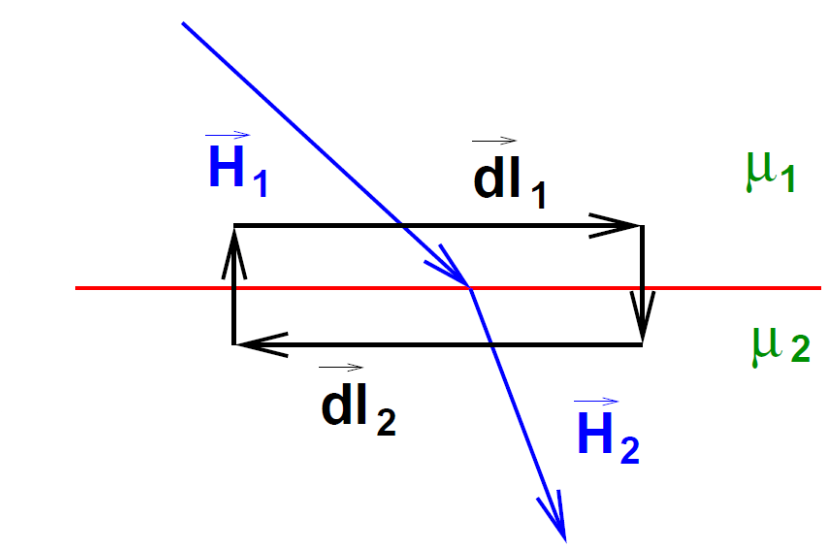
\includegraphics[width=0.95\textwidth]{./images/schematics/boundary_conditions_magnetic_field_2.png}\\
    \end{center}
  \end{column}
\end{columns}

\begin{equation*}
  \oint \vec{H} \cdot d\vec{\ell} = 0 \Rightarrow
       %\vec{H}_1 \vec{\ell}_1 + \vec{H}_2 \vec{\ell}_2 = 0 \Rightarrow
       H_1^{\parallel} \ell - H_2^{\parallel} \ell = 0 \Rightarrow
        {\color{magenta} H_1^{\parallel} = H_2^{\parallel}}
\end{equation*}

The magnetizing field $\vec{H}$ is given by
$\displaystyle \vec{H} = \frac{1}{\mu} \vec{B}$,
therefore:
\begin{equation*}
        {\color{magenta} \frac{1}{\mu_1}  B_1^{\parallel} = \frac{1}{\mu_2} B_2^{\parallel}}
\end{equation*}

\end{frame}


%
%
%

\begin{frame}{Boundary conditions: Summary}

For the electric field:
{\Large
\begin{equation*}
    \epsilon_1 E_1^{\perp} = \epsilon_2 E_2^{\perp}
\end{equation*}
\vspace{0.1cm}
\begin{equation*}
    E_1^{\parallel} = E_2^{\parallel}
\end{equation*}
}

\vspace{0.2cm}

For the magnetic field:
{\Large
\begin{equation*}
    B_1^{\perp} = B_2^{\perp}
\end{equation*}
\vspace{0.1cm}
\begin{equation*}
    \frac{1}{\mu_1} B_1^{\parallel} = \frac{1}{\mu_2} B_2^{\parallel}
\end{equation*}
}

\end{frame}


%
% Worked example
%

{
\problemslide

%
%
%

\begin{frame}{Worked example}

\begin{blockexmplque}{Question}
\begin{columns}
  \begin{column}{0.25\textwidth}
   \begin{center}
     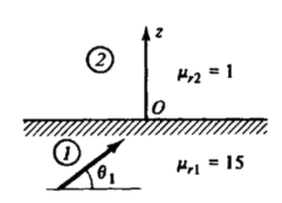
\includegraphics[width=0.98\textwidth]{./images/problems/lect8_boundary.png}
   \end{center}
  \end{column}
  \begin{column}{0.75\textwidth}
     In region 1, $\displaystyle \vec{B}_1 = \Big(1.2, 0.8, 0.4 \Big)$ T.
     Find $\vec{H}_2$ at z=0. \\
     Calculate the angles between the B field vectors and a tangent to the
     interface between the two regions.
  \end{column}
\end{columns}

\end{blockexmplque}

\vspace{0.2cm}

Recall that: $\displaystyle H = \frac{B}{\mu} = \frac{B}{\mu_r \mu_0}$

\vspace{0.4cm}

The relevenant electrodynamic boundary conditions are:
\begin{equation*}
  B_1^{\perp} = B_2^{\perp} \;\;\;\; and \;\;\;\;
  H_1^{\parallel} = H_2^{\parallel} \Rightarrow  \frac{1}{\mu_1}  B_1^{\parallel} = \frac{1}{\mu_2} B_2^{\parallel}
\end{equation*}

\end{frame}

%
%
%

\begin{frame}{Worked example}

Therefore:\\
\vspace{0.2cm}

\begin{itemize}
\item
   $\displaystyle \vec{B}_1 = \Big(1.2, 0.8, 0.4 \Big)$ T
\item
   $\displaystyle \vec{H}_1 = \frac{1}{\mu_0} \Big(8.0, 5.33, 2.67 \Big) \cdot 10^{-2}$ A/m
\item
   $\displaystyle \vec{H}_2 = \frac{1}{\mu_0} \Big(8.0, 5.33, 10^{2} \mu_0 H_{z2} \Big) \cdot 10^{-2}$ A/m
\item
   $\displaystyle \vec{B}_2 = \Big(B_{x2}, B_{y2}, 0.4 \Big)$ T
\end{itemize}

\vspace{0.2cm}

The remaining unknown terms follow directly:
\begin{equation*}
  B_{x2} = \mu_0 \cdot \mu_{r2} \cdot H_{x2} = 8.0 \times 10^{-2} \; T
\end{equation*}
\begin{equation*}
  B_{y2} = 5.33 \times 10^{-2} \; T
\end{equation*}
\begin{equation*}
  H_{z2} = \frac{H_{z2}}{\mu_0 \cdot \mu_{r2}} = \frac{0.4}{\mu_0} \; A/m
\end{equation*}

\end{frame}

%
%
%

\begin{frame}{Worked example}

Angle $\theta_1$ is $90^{o}-\alpha_1$ where $\alpha_1$ is the angle between $B_1$ and $\hat{z}=\Big(0,0,1\Big)$.
\begin{equation*}
  cos\alpha_1 = \frac{ \vec{B}_1 \cdot \hat{z} }{|\vec{B}_1|} = 0.27 \Rightarrow \alpha_1 = 74.5^{o}
\end{equation*}
and therefore:
\begin{equation*}
  \theta_1 = 90^{o}-74.5^{o} \Rightarrow  \theta_1 = 15.5^{o}.
\end{equation*}

Similarly, $\theta_2 = 76.5^{o}$.

\end{frame}

} % end of worked example



%
%
%

\begin{frame}{Reflection and transmission (refraction)}

\begin{columns}
  \begin{column}{0.40\textwidth}
      Consider a wave (incident wave) hitting the boundary
      between two linear transparent media.\\
      \vspace{0.2cm}
      This gives rise to a {\bf reflected} and a {\bf transmitted} wave.\\
      \vspace{0.2cm}
      I would like to calculate the intensity of the reflected and
      transmitted waves.\\
  \end{column}
  \begin{column}{0.60\textwidth}
    \begin{center}
      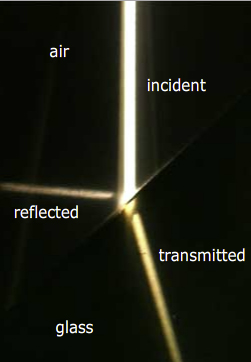
\includegraphics[width=0.66\textwidth]{./images/photos/still_interference_refraction.png}\\
    \end{center}
  \end{column}
\end{columns}


\end{frame}

%
%
%

\begin{frame}{Reflection and transmission at normal incidence}

Suppose the xy plane is the boundary between two linear media.\\
\vspace{0.2cm}
A plane wave of frequency $\omega$, travelling in the +z direction and
polarized in the x direction approached the boundary from the left.

\begin{columns}
  \begin{column}{0.40\textwidth}
  {\Large
   \begin{equation*}
        \vec{E}_I (z,t) = {E_I}_0  e^{i (k_1 z-\omega t)}  \hat{x}
   \end{equation*}
   \vspace{0.3cm}
   \begin{equation*}
         \vec{B}_I (z,t) = \frac{{E_I}_0}{u_1}  e^{i (k_1 z-\omega t)} \hat{y}
    \end{equation*}
  }
  \end{column}
  \begin{column}{0.60\textwidth}
    \begin{center}
      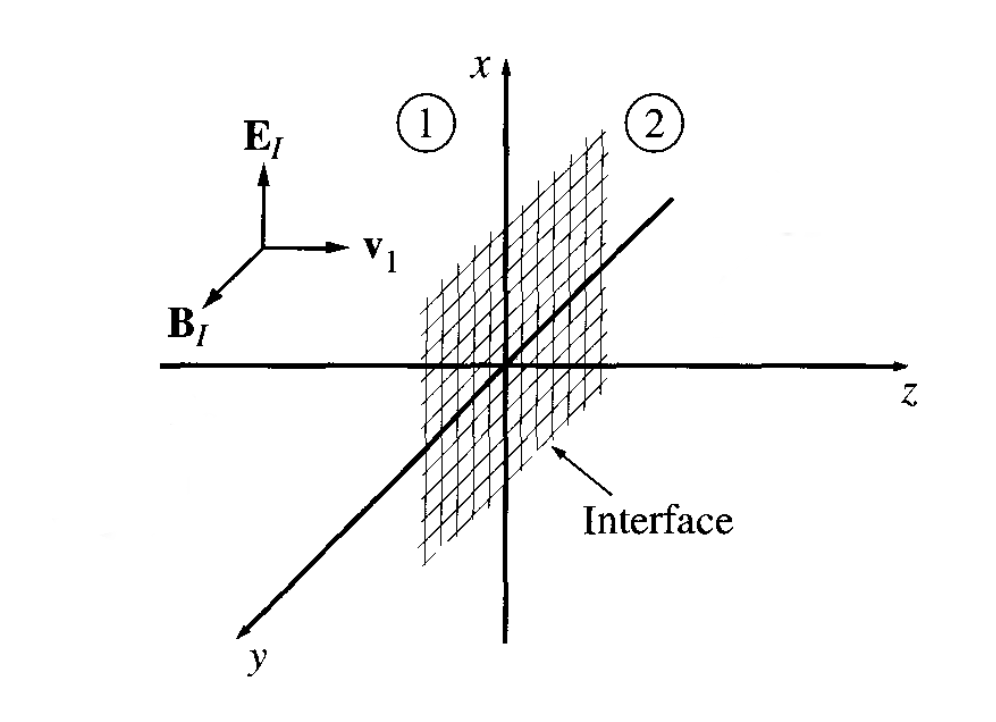
\includegraphics[width=0.99\textwidth]{./images/schematics/wave_reflection_transmission_normal_incidence_1.png}\\
    \end{center}
  \end{column}
\end{columns}

\end{frame}

%
%
%

\begin{frame}{Reflection and transmission at normal incidence}

This gives rise to a {\bf reflected} and a {\bf transmitted} wave.\\
\begin{center}
    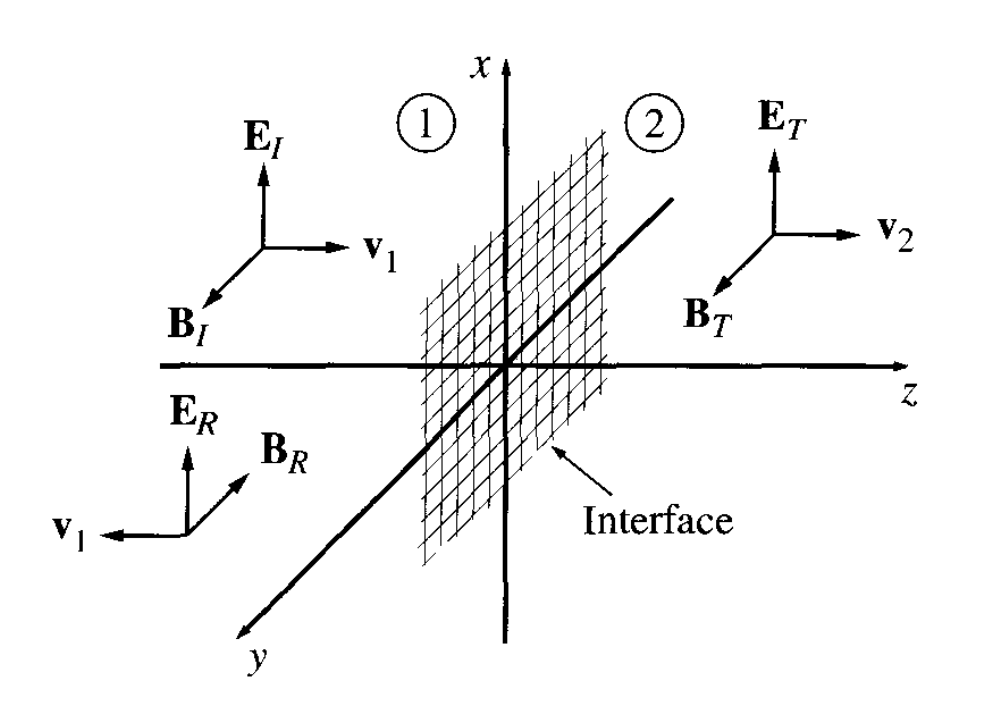
\includegraphics[width=0.80\textwidth]{./images/schematics/wave_reflection_transmission_normal_incidence_2.png}\\
\end{center}

\end{frame}


%
%
%

\begin{frame}{Reflection and transmission at normal incidence}

\begin{columns}
  \begin{column}{0.40\textwidth}
     Reflected wave:
     \begin{equation*}
          \vec{E}_R (z,t) = {E_R}_0  e^{i (-k_1 z-\omega t)}  \hat{x}
      \end{equation*}
     \begin{equation*}
          \vec{B}_R (z,t) = -\frac{{E_R}_0}{u_1}  e^{i (-k_1 z-\omega t)} \hat{y}
      \end{equation*}\\
      \vspace{0.4cm}
      Transmitted wave:
      \begin{equation*}
           \vec{E}_T (z,t) = {E_T}_0  e^{i ( k_2 z-\omega t)}  \hat{x}
       \end{equation*}
      \begin{equation*}
           \vec{B}_T (z,t) = \frac{{E_T}_0}{u_2}  e^{i (k_2 z-\omega t)} \hat{y}
       \end{equation*}
  \end{column}
  \begin{column}{0.60\textwidth}
    \begin{center}
      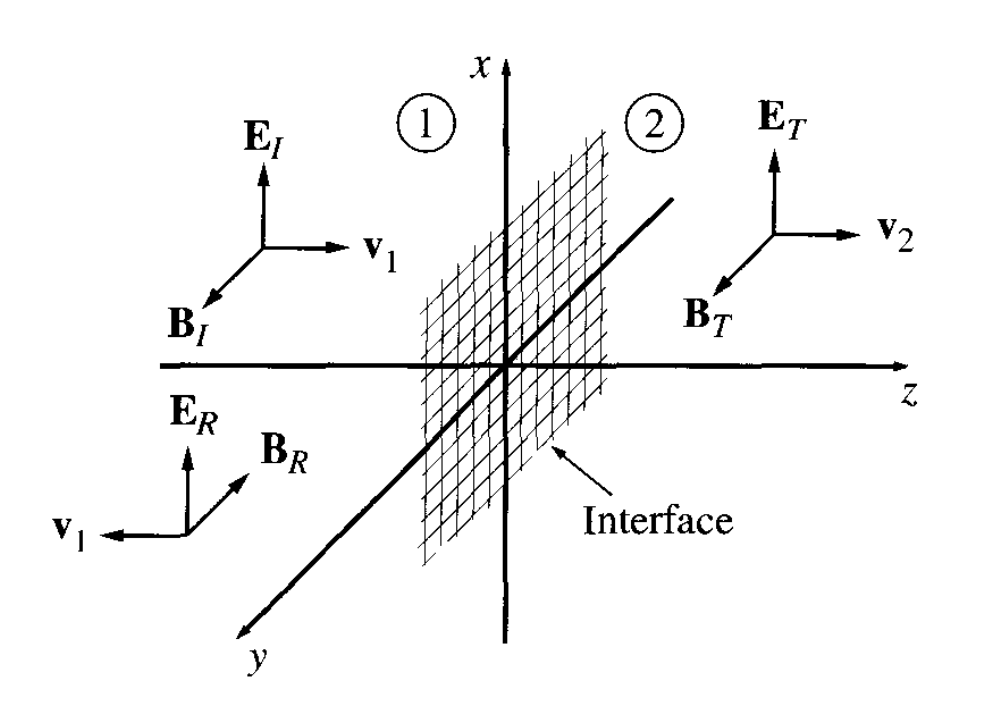
\includegraphics[width=0.99\textwidth]{./images/schematics/wave_reflection_transmission_normal_incidence_2.png}\\
    \end{center}
  \end{column}
\end{columns}

\vspace{0.4cm}

\noindent\rule{2cm}{0.4pt}\\
{\scriptsize
  Notice that if the incident wave travels along the propagation vector $\vec{k}$,
  the reflected wave (for normal incidence) travels along $-\vec{k}$.
  Also, notice the change of sign of $\vec{B}_R$
  as required by $\displaystyle \vec{B}_{0} = \frac{1}{\omega} \Big( \vec{k} \times \vec{E}_0 \Big)$
  (see earlier in this lecture).\\
}

\end{frame}

%
%
%

\begin{frame}{Reflection and transmission at normal incidence}

\begin{itemize}
         \item On the right of the boundary (2) there is only the transmitted wave::
              \begin{equation*}
                  \vec{E}_2 = \vec{E}_T \;\;\; and \;\;\; \vec{B}_2 = \vec{B}_T
              \end{equation*}
         \item On the left of the boundary (1)  we have both the incoming and reflected waves:
              \begin{equation*}
                  \vec{E}_1 = \vec{E}_I + \vec{E}_R \;\;\; and \;\;\; \vec{B}_1 = \vec{B}_I + \vec{B}_R
              \end{equation*}
\end{itemize}

At z=0 (boundary between the two linear media), the following
boundary conditions should be satisfied:
\begin{equation*}
    \cancel{\epsilon_1 E_1^{\perp} = \epsilon_2 E_2^{\perp}}
    \;\;\; and \;\;\;
    E_1^{\parallel} = E_2^{\parallel}
\end{equation*}
\begin{equation*}
    \cancel{B_1^{\perp} = B_2^{\perp}}
    \;\;\; and \;\;\;
    \frac{1}{\mu_1} B_1^{\parallel} = \frac{1}{\mu_2} B_2^{\parallel}
\end{equation*}

\noindent\rule{2cm}{0.4pt}\\
{\scriptsize
  In this case there are {\bf no field components perpendicular to the surface},
  so the corresponding boundary conditions are trivially satisfied.

}

\end{frame}

%
%
%

\begin{frame}{Reflection and transmission at normal incidence}

Will examine what we learn from the $E_1^{\parallel} = E_2^{\parallel}$ boundary condition:

\begin{equation*}
    E_1^{\parallel}(z=0, t) = E_2^{\parallel}(z=0, t) \Rightarrow
\end{equation*}

\begin{equation*}
    \vec{E}_I(z=0, t) + \vec{E}_R(z=0, t)  = \vec{E}_T(z=0, t)  \Rightarrow
\end{equation*}

\begin{equation*}
    {E_I}_0  e^{-i \omega t}  \hat{x} +  {E_R}_0  e^{-i \omega t}  \hat{x} =
    {E_T}_0  e^{-i \omega t}  \hat{x}  \Rightarrow
\end{equation*}

\begin{equation*}
    \Big( {E_I}_0 + {E_R}_0  \Big) \cancel{e^{-i \omega t}  \hat{x}} =
    {E_T}_0  \cancel{e^{-i \omega t}  \hat{x}}  \Rightarrow
\end{equation*}

\begin{equation*}
    {\color{magenta}
       {E_I}_0  +  {E_R}_0  = {E_T}_0
    }
\end{equation*}

\end{frame}

%
%
%

\begin{frame}{Reflection and transmission at normal incidence}

Will also examine what we learn from the
$\frac{1}{\mu_1} B_1^{\parallel} = \frac{1}{\mu_2} B_2^{\parallel}$ condition:

\begin{equation*}
    \frac{1}{\mu_1} B_1^{\parallel}(z=0, t) = \frac{1}{\mu_2} B_2^{\parallel}(z=0, t) \Rightarrow
\end{equation*}

\begin{equation*}
    \frac{1}{\mu_1} \Big( \vec{B}_I(z=0, t) + \vec{B}_R(z=0, t) \Big) = \frac{1}{\mu_2} \vec{B}_T(z=0, t) \Rightarrow
\end{equation*}

\begin{equation*}
    \frac{1}{\mu_1}
      \Big( \frac{{E_I}_0}{u_1}   e^{-i \omega t} \hat{y}
             -\frac{{E_R}_0}{u_1}  e^{-i \omega t} \hat{y}
       \Big) = \frac{1}{\mu_2} \frac{{E_T}_0}{u_2}  e^{-i \omega t} \hat{y} \Rightarrow
\end{equation*}

\begin{equation*}
    \frac{1}{\mu_1 u_1} \Big( {E_I}_0 - {E_R}_0 \Big) \cancel{e^{-i \omega t} \hat{y}} =
    \frac{1}{\mu_2 u_2}  {E_T}_0  \cancel{e^{-i \omega t} \hat{y}} \Rightarrow
\end{equation*}

\begin{equation*}
    {\color{magenta}
      \frac{1}{\mu_1 u_1} \Big( {E_I}_0 - {E_R}_0 \Big) = \frac{1}{\mu_2 u_2}  {E_T}_0
    }
\end{equation*}

\end{frame}

%
%
%

\begin{frame}{Reflection and transmission at normal incidence}

The two boundary conditions led to the following system of equations:
\begin{equation*}
   {E_I}_0  +  {E_R}_0  = {E_T}_0  \;\;\; and \;\;\;
   \frac{1}{\mu_1 u_1} \Big( {E_I}_0 - {E_R}_0 \Big) = \frac{1}{\mu_2 u_2}  {E_T}_0
\end{equation*}

Solving that system for ${E_R}_0$ and ${E_T}_0$ we get:
\begin{equation*}
    {\color{magenta}
         {E_R}_0 = \frac{1-\beta}{1+\beta} {E_I}_0
    }
\end{equation*}

\begin{equation*}
    {\color{magenta}
         {E_T}_0 = \frac{2}{1+\beta} {E_I}_0
    }
\end{equation*}

where
\begin{equation*}
  \beta = \frac{\mu_1 u_1}{\mu_2 u_2} = \frac{\mu_1 n_2}{\mu_2 n_1}
\end{equation*}

\end{frame}

%
%
%

\begin{frame}{Reflection and transmission coefficients}

We define the reflection (transmission) coefficient using the ratio of
the reflected (transmitted) intensity
with the incident amplitude.\\
\vspace{0.2cm}
Reflection coefficient R:
\begin{equation*}
   R = \frac{I_R}{I_I}
\end{equation*}
\vspace{0.2cm}
Transmission coefficient T:
\begin{equation*}
   T = \frac{I_T}{I_I}
\end{equation*}


\noindent\rule{2cm}{0.4pt}\\
{ \small
  For a monochromatic plane wave
  with an electric field amplitude $E_0$,
  propagating with velocity u within a medium with permittivity (permeability) $\epsilon$ ($\mu$),
  the intensity I  (average power per unit area) is given by
  \begin{equation*}
      I = \frac{1}{2\mu u} E_0^2 = \frac{1}{2} \epsilon u E_0^2
  \end{equation*}
}

\end{frame}

%
%
%

\begin{frame}{Reflection and transmission coefficients}

\begin{equation*}
   R = \frac{I_R}{I_I} =
          \frac{ \cancel{ \frac{1}{2} \epsilon_1 u_1} {E_R}_0^2}{ \cancel{ \frac{1}{2} \epsilon_1 u_1} {E_I}_0^2} =
          \Big( \frac{ {E_R}_0 } { {E_I}_0} \Big)^2 =
          \Big( \frac{1-\beta}{1+\beta} \Big)^2
          \xRightarrow{\beta \approx n_2/n_1}
\end{equation*}
\begin{equation*}
{\color{magenta}
   R = \Big( \frac{n_1-n_2}{n_1+n_2} \Big)^2
}
\end{equation*}

\vspace{0.1cm}

\begin{equation*}
   T = \frac{I_T}{I_I} =
          \frac{ \cancel{ \frac{1}{2} \epsilon_2 u_2} {E_T}_0^2}{ \cancel{ \frac{1}{2} \epsilon_1 u_1} {E_I}_0^2} =
          \frac{\epsilon_2 u_2}{\epsilon_1 u_1} \Big( \frac{{E_T}_0}{{E_I}_0} \Big)^2 =
          \frac{\epsilon_2 u_2}{\epsilon_1 u_1}\Big( \frac{2}{1+\beta} \Big)^2 \;\;
          \xRightarrow{\beta \approx n_2/n_1}
\end{equation*}
\begin{equation*}
   T = \frac{\epsilon_2 u_2}{\epsilon_1 u_1} \frac{4 n_1^2}{(n_1+n_2)^2}
          \xRightarrow{\displaystyle \small \frac{\epsilon_2 u_2}{\epsilon_1 u_1} = \frac{\mu_1 u_1^2 u_2}{\mu_2 u_2^2 u_1} \approx u_1/u_2 = n_2/n_1}
\end{equation*}
\begin{equation*}
{\color{magenta}
    T = \frac{4 n_1 n_2}{(n_1+n_2)^2}
}
\end{equation*}

\end{frame}


\begin{frame}{Reflection and transmission coefficients}

So, for example, for an EM wave crossing the boundary between a volume of air ($n_1$=1)
and a glass ($n_2$=1.5):
\vspace{0.2cm}
\begin{itemize}
  \item $\displaystyle R = \Big( \frac{n_1-n_2}{n_1+n_2} \Big)^2 = \Big( \frac{1-1.5}{1+1.5} \Big)^2 = 4\%$
   \vspace{0.2cm}
  \item $\displaystyle T =  \frac{4 n_1 n_2}{(n_1+n_2)^2} =  \frac{4 \cdot 1.5}{(1+1.5)^2} = 96\%$
\end{itemize}

\vspace{0.4cm}

We can easily confirm that
\begin{equation*}
  R + T = 1
\end{equation*}
as a consequence of the conservation of energy.

\end{frame}

%
%
%

\begin{frame}{Reflection and transmission at oblique incidence}

\begin{columns}
  \begin{column}{0.66\textwidth}
   {\small
     General case of {\em oblique} incidence:
     \begin{itemize}
     {\small
        \item Incoming wave meets the boundary plane at an arbitrary angle $\theta_I$.
        \item The angle of transmission (or refraction) is $\theta_T$.
        \item The angle of reflection is $\theta_R$.
     }
     \end{itemize}
   }
  \end{column}
  \begin{column}{0.34\textwidth}
    \begin{center}
      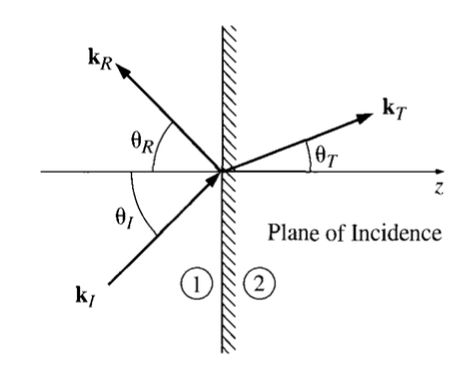
\includegraphics[width=0.99\textwidth]{./images/schematics/wave_reflection_transmission_oblique_incidence.png}\\
    \end{center}
  \end{column}
\end{columns}

The analysis is {\bf similar as before}, but the algebra is slightly more complex.\\
\vspace{0.2cm}
{\bf Study this case on your own}.\\

\end{frame}

%
%
%

\begin{frame}{Reflection and transmission at oblique incidence}

The analysis of reflection and transmission at oblique incidence
leads to the three known laws of geometrical optics:

\begin{itemize}
  \item {\bf 1$^{st}$ Law}:\\
     The incident, reflected, and transmitted wave vectors form a plane (plane of incidence),
     which also includes the normal to the surface.
     \begin{equation*}
          k_I sin\theta_I = k_R sin\theta_R = k_T sin\theta_T
      \end{equation*}
  \item {\bf 2$^{nd}$ Law} ({\bf Law of reflection}):\\
     The angle of incidence is equal to the angle of reflection.
     \begin{equation*}
          \theta_I = \theta_R
      \end{equation*}
  \item {\bf 3$^{rd}$ Law} ({\bf Law of refraction} or {\bf Snell's law}):\\
     \begin{equation*}
          \frac{sin\theta_T}{sin\theta_I} = \frac{n_1}{n_2}
      \end{equation*}

\end{itemize}

\end{frame}

%
%
%

\begin{frame}{Refraction}

\begin{columns}
  \begin{column}{0.66\textwidth}
   \begin{center}
      {\bf Law of refraction} or {\bf Snell's law}:
     \begin{equation*}
          n_1 sin\theta_1 = n_2 sin\theta_2
      \end{equation*}
   \end{center}
  \end{column}
  \begin{column}{0.34\textwidth}
    \begin{center}
      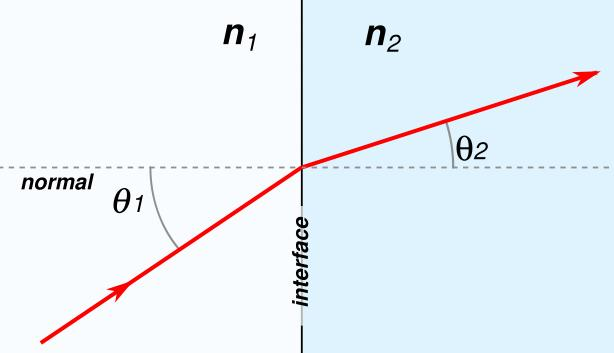
\includegraphics[width=0.75\textwidth]{./images/schematics/snells_law}\\
    \end{center}
  \end{column}
\end{columns}

\vspace{0.2cm}

\begin{center}
    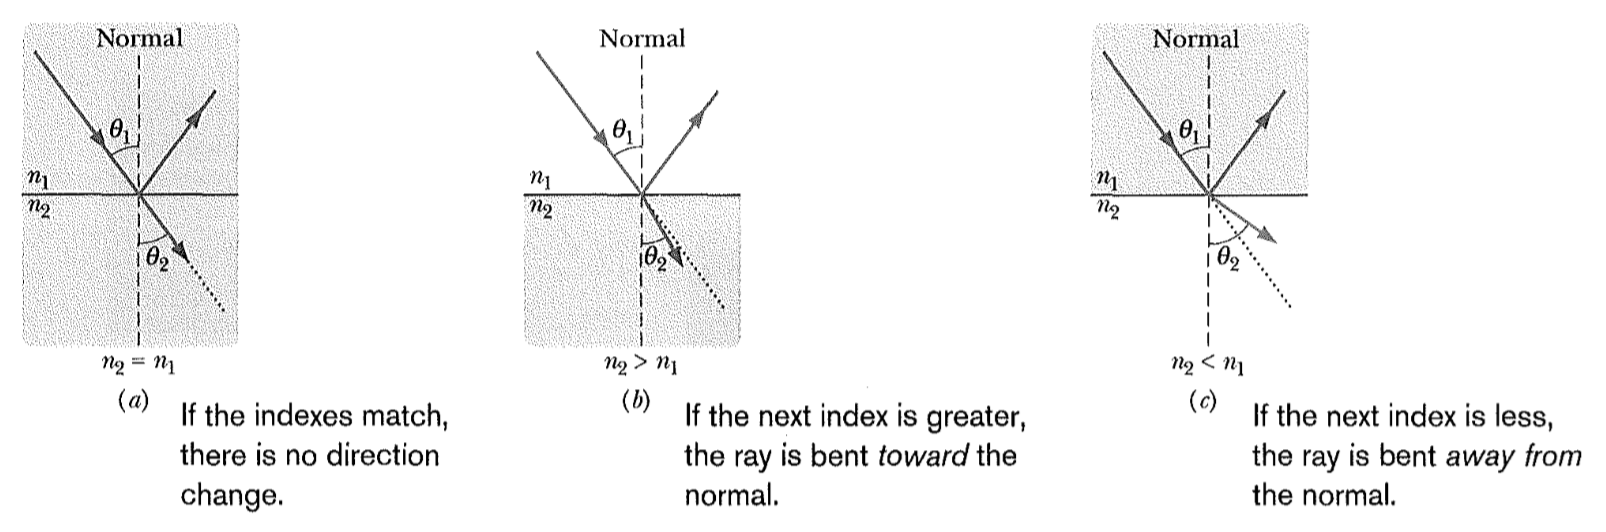
\includegraphics[width=0.99\textwidth]{./images/schematics/refraction_direction}\\
\end{center}

\end{frame}



%
% Worked example
%

{
\problemslide

%
%
%

\begin{frame}{Worked example}

\begin{blockexmplque}{Question}
\begin{columns}
  \begin{column}{0.25\textwidth}
   \begin{center}
     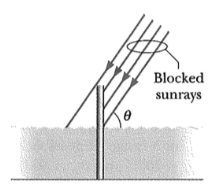
\includegraphics[width=0.90\textwidth]{./images/problems/lect8_pole_shadow.png}
   \end{center}
  \end{column}
  \begin{column}{0.75\textwidth}
     A 2.0-m-long vertical rod is extending
     from the bottom of a water tank to a point 50 cm above the surface
     of the water. The bottom of the water tank is level.
     Sunlight is incident at angle $\theta$=55$^{o}$. What
     is the length of the shadow of the rod at the bottom of the tank?
  \end{column}
\end{columns}
The index of refraction for air (water) is 1 (1.33).
\end{blockexmplque}

\vspace{0.2cm}

\begin{columns}
  \begin{column}{0.25\textwidth}
   \begin{center}
     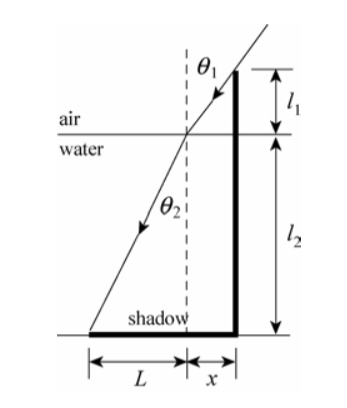
\includegraphics[width=0.95\textwidth]{./images/problems/lect8_pole_shadow_solution.png}
   \end{center}
  \end{column}
  \begin{column}{0.75\textwidth}
     Consider a ray that grazes the top of the rod, as shown.\\
     \vspace{0.2cm}
     Here $\theta_1 = 90^{o}-\theta= 35^{o}$, $l_1$ =0.50 m, and $l_2$=1.50 m.\\
     \vspace{0.2cm}
    The length of the shadow is x + L.\\
  \end{column}
\end{columns}

\end{frame}

%
%
%

\begin{frame}{Worked example}

The distance x is given by:
\begin{equation*}
    x=l_1 \cdot tan\theta_1 = (0.50 \; m) \cdot tan35^{o} = 0.35 m
\end{equation*}

According to the law of refraction:
\begin{equation*}
   n_2 \cdot  sin\theta_2 = n_1 \cdot sin\theta_1
\end{equation*}

Therefore:
\begin{equation*}
  \theta_2 = sin^{-1} \Big( \frac{n_1}{n_2} \cdot sin\theta_1 \Big)
                = sin^{-1} \Big( \frac{1}{1.33} \cdot sin35.0^{o} \Big) \Rightarrow \theta_2 = 25.54^{o}
\end{equation*}

The distance L is given by:
\begin{equation*}
   L = l_2 \cdot tan\theta_2 = (1.50\; m) \cdot tan25.54^{o} = 0.72 \; m
\end{equation*}

The length of the shadow is: 0.35 m  + 0.72 m = 1.07 m.

\end{frame}

} % end of worked example

%
%
%

\begin{frame}{Total internal reflection}

As the angle of incidence increases, the angle of refraction
increases: For some critical value $\theta_c$, the angle of refraction
becomes 90$^o$.\\
\vspace{0.1cm}
For angles of incidence larger than $\theta_c$, such as for rays f and
g below, there is no refracted ray and all the light is reflected;
this effect is called {\bf total internal reflection}.\\
\begin{equation*}
       n_1 sin\theta_c = n_2 sin90^o \Rightarrow
       {\color{magenta}\theta_c = sin^{-1} \frac{n_2}{n_1}}\;\;\;\;\;(n_2 < n_1)
\end{equation*}

\begin{center}
    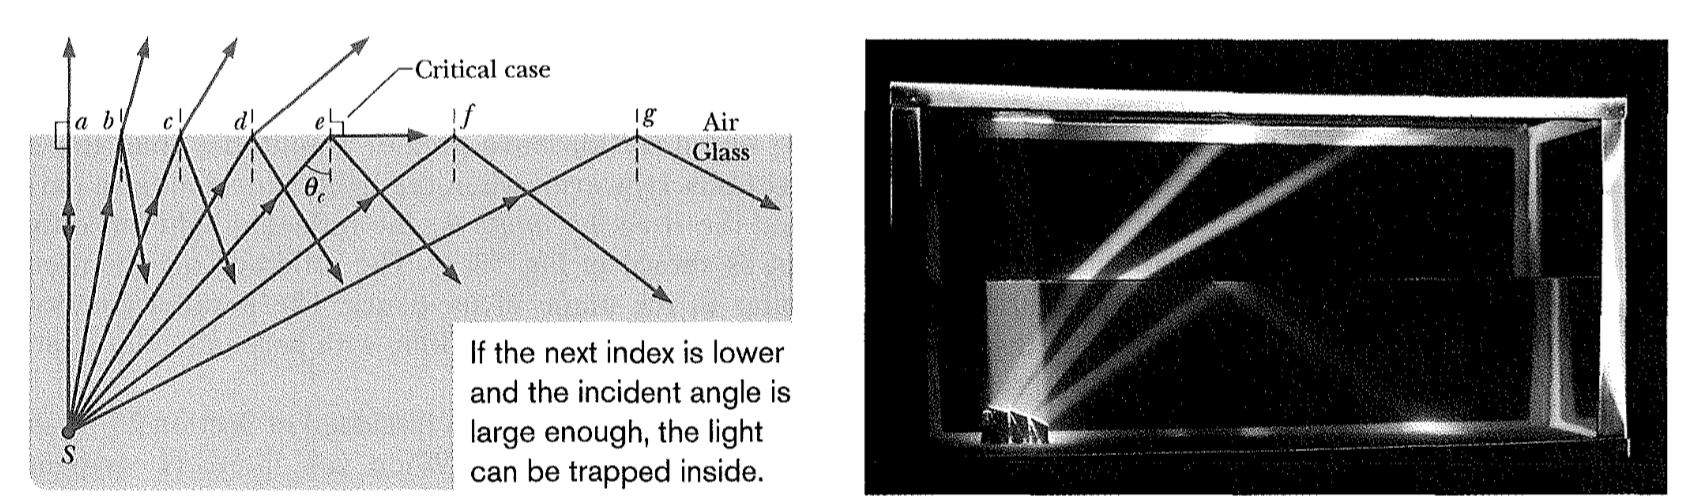
\includegraphics[width=0.95\textwidth]{./images/schematics/total_internal_reflection}\\
\end{center}

\end{frame}

%
%
%

\begin{frame}{Total internal reflection}

Consider how a fish sees the world outside the water: A `circle of light'

\begin{center}
    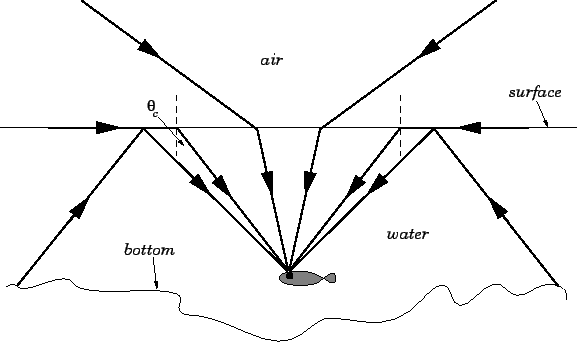
\includegraphics[width=0.75\textwidth]{./images/schematics/fish_view_circle_of_light}\\
\end{center}

Use this schematic for the workshop tomorrow!

\end{frame}

%
%
%

\begin{frame}{Polarisation by reflection}

\begin{itemize}
 \item
     A randomly polarised wave: the sum of a wave polarised
     on the incidence plane and one polarised perpendicularly to it.
    \begin{itemize}
       \item
          For unpolarized light, these two components are of equal magnitude.
    \end{itemize}
  \item
      In general, the reflected light also has both components but
      with unequal magnitudes:
      the {\bf reflected light is partially polarized}
\end{itemize}

\begin{columns}
  \begin{column}{0.30\textwidth}
   \begin{center}
      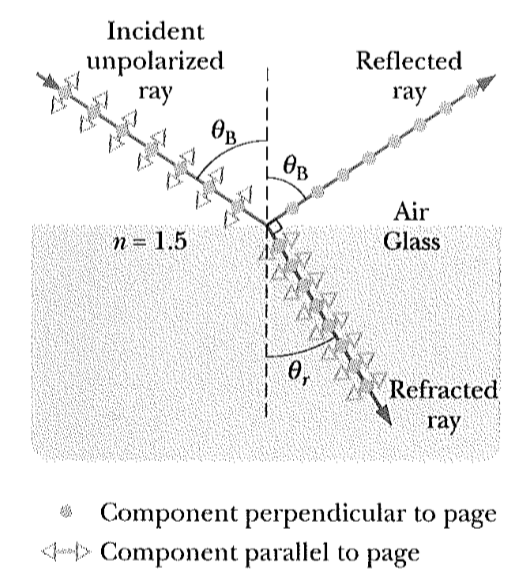
\includegraphics[width=0.99\textwidth]{./images/schematics/polarization_by_reflection}\\
   \end{center}
  \end{column}
  \begin{column}{0.70\textwidth}
   \begin{itemize}
    \item
     When the light is incident at a particular incident angle, called {\bf Brewster angle}
     given by:
     \begin{equation*}
          tan\theta_B \approx \frac{n_2}{n_1}
      \end{equation*}
      The reflected light has only perpendicular components: It is
      {\bf fully polarized} perpendicular to the plane of incidence.
    \item
       For light incident at that angle, the reflected and refracted rays are perpendicular to each other.
   \end{itemize}
  \end{column}
\end{columns}

\end{frame}


% ------------------------------------------------------------------------------
% ------------------------------------------------------------------------------

%
% What to remember
%

\renewcommand{\lecturesummarytitle}{Main points to remember }

\renewcommand{\summarizedlecture}{10 }

%
%
%

\begin{frame}{Lecture \summarizedlecture - \lecturesummarytitle}

{\small

We studied the most general case of Maxwell's equations:\\

\setlength{\extrarowheight}{12pt}
\setlength{\arraycolsep}{5pt}

 \begin{center}
 {

  \begin{table}[H]
    \begin{tabular}{|l|c|c|}
      \hline
        \multicolumn{3}{|l|} {
          {\color{magenta}
           {\bf Dynamic case in matter}
          }
        }\\
      \hline
      {\bf Gauss's law} &
        $\displaystyle \oint \vec{D} d\vec{S} = \int \rho_f d\tau = Q_f$   &
        $\displaystyle \vec{\nabla} \cdot \vec{D} = \rho_f$ \\

      {\bf Faraday's law} &
        $\displaystyle \oint \vec{E} d\vec{\ell} = -\frac{\partial}{\partial t} \int \vec{B} d\vec{S} \Rightarrow$ &
        $\displaystyle \vec{\nabla} \times \vec{E} = -  \frac{\partial \vec{B}}{\partial t}$ \\
      &
        $\displaystyle \oint \vec{E} d\vec{\ell} = -\frac{d\Phi_B}{dt}$ & \\

      no magn. monopoles &
        $\displaystyle  \oint \vec{B} d\vec{S} = 0$ &
        $\displaystyle  \vec{\nabla} \cdot \vec{B} = 0$ \\

      {\bf Ampere's law} &
        $\displaystyle \oint \vec{H} d\vec{\ell} = \int_{S} \Big( \vec{j} + \frac{\partial \vec{D}}{\partial t}\Big) d\vec{S} \Rightarrow$ &
        $\displaystyle \vec{\nabla} \times \vec{H} = \vec{j}_f + \frac{\partial \vec{D}}{\partial t}$ \\
      &
        $\displaystyle \oint \vec{H} d\vec{\ell} = I_f + \frac{d\Phi_D}{dt}$ & \\
      \hline
    \end{tabular}
  \end{table}

 }
 \end{center}
}

\end{frame}

%
%
%

\begin{frame}{Lecture \summarizedlecture - \lecturesummarytitle (cont'd)}

\begin{itemize}

\item As we did in vacuum, we studied Maxwell's equations in matter (for time-dependent fields)
          and in the absence of sources and we saw that they give rise to EM waves:
          \begin{equation*}
             \vec{\nabla}^{2} \vec{E} = \mu \epsilon \frac{\partial^{2} \vec{E}}{\partial t^{2}} \;\;\;\; and \;\;\;\;
             \vec{\nabla}^{2} \vec{B} = \mu \epsilon \frac{\partial^{2} \vec{B}}{\partial t^{2}}
         \end{equation*}

\item Speed of EM waves in matter: $\displaystyle u = \frac{1}{\sqrt{\epsilon \mu}}$
         \begin{itemize}
         {\small
               \item EM waves in matter propagate slower than EM waves in vacuum
               \item $\displaystyle u = \frac{c}{n}$ where
                         $\displaystyle n = \frac{\sqrt{\epsilon \mu}}{\sqrt{\epsilon_0 \mu_0}}$
                         is the index of refraction of the material.
         }
         \end{itemize}

\item We introduced a complex representation of EM waves starting from de Moivre's theorem
          and embedding the known EM wave properties (EM waves are always {\bf transverse} and
          {\bf mutually perpendicular}):
          \begin{equation*}
                \vec{E}(\vec{r},t) = E_0  e^{i (\vec{k} \vec{r} -\omega t)} \hat{n}
                 \;\;\; and \;\;\;
                \vec{B}(\vec{r},t) =
                  \frac{E_0}{c}  e^{i ( \vec{k} \vec{r} -\omega t)} \Big( \hat{k} \times \hat{n} \Big) =
                  \frac{1}{c}  \Big( \hat{k} \times \vec{E} \Big)
          \end{equation*}

\end{itemize}

\end{frame}

%
%
%

\begin{frame}{Lecture \summarizedlecture - \lecturesummarytitle (cont'd)}

\begin{itemize}

\item We also studied EM wave polarization and practical applications.

\item Finally, we studied the electrodynamic boundary conditions:\\
          \vspace{0.2cm}
         For the electric field:
         \begin{equation*}
               \epsilon_1 E_1^{\perp} = \epsilon_2 E_2^{\perp}  \;\;\;\; and \;\;\;\;
                E_1^{\parallel} = E_2^{\parallel}
         \end{equation*}
         For the magnetic field:
         \begin{equation*}
               B_1^{\perp} = B_2^{\perp} \;\;\;\; and \;\;\;\;
               \frac{1}{\mu_1} B_1^{\parallel} = \frac{1}{\mu_2} B_2^{\parallel}
         \end{equation*}

\item We used the above conditions to study what happens when
          an EM wave crosses the {\bf boundary between two transparent media}\\
          \vspace{0.2cm}
          Two cases:
          \begin{itemize}
               \item Normal incidence
               \item Oblique incidence (general case / home study)
          \end{itemize}
\end{itemize}

\end{frame}


%
%
%

\begin{frame}{Lecture \summarizedlecture - \lecturesummarytitle (cont'd)}

\begin{itemize}
{\small
\item Maxwell's equations in most general form (time-dependent fields in matter)
    \begin{itemize}
     {\scriptsize
          \item You should know both the integral and differential forms.
          \item You should know all variations of these equations and be able to derive
                    one from another (dynamic $\rightarrow$ static, matter $\rightarrow$ vacuum)
          \item No marks given for writing the wrong set of equations, even if they are all
                    similar and interconnected.\\
    }
    \end{itemize}

\item You should be able to show that Maxwell's equations (in vacuum or in matter) in
          absence of sources describe EM waves

\item You should know how the wave equation and the EM waves are different in vacuum and in transparent media.

\item You should know how to use the complex representation of waves.

\item You should know (and be able to derive) the electrodynamic boundary conditions,
          and you should be able to use them to study reflection and transmission at normal and oblique incidence.

\item You should remember the fundamental laws of geometrical optics and what is Brewster's angle.
}
\end{itemize}

\end{frame}


%
% Plan for the next lecture
%

\begin{frame}{Plan for Lecture \nextlecture}

\begin{itemize}
\item Mutual and self inductance
\vspace{0.2cm}
\item Inductance in circuits
  \begin{itemize}
      \item RL circuits
      \item LC circuits
      \item RLC circuits
  \end{itemize}
\end{itemize}

\end{frame}

% ------------------------------------------------------------------------------
% ------------------------------------------------------------------------------
